\PassOptionsToPackage{unicode=true}{hyperref} % options for packages loaded elsewhere
\PassOptionsToPackage{hyphens}{url}
%
\documentclass[]{book}
\usepackage{lmodern}
\usepackage{amssymb,amsmath}
\usepackage{ifxetex,ifluatex}
\usepackage{fixltx2e} % provides \textsubscript
\ifnum 0\ifxetex 1\fi\ifluatex 1\fi=0 % if pdftex
  \usepackage[T1]{fontenc}
  \usepackage[utf8]{inputenc}
  \usepackage{textcomp} % provides euro and other symbols
\else % if luatex or xelatex
  \usepackage{unicode-math}
  \defaultfontfeatures{Ligatures=TeX,Scale=MatchLowercase}
\fi
% use upquote if available, for straight quotes in verbatim environments
\IfFileExists{upquote.sty}{\usepackage{upquote}}{}
% use microtype if available
\IfFileExists{microtype.sty}{%
\usepackage[]{microtype}
\UseMicrotypeSet[protrusion]{basicmath} % disable protrusion for tt fonts
}{}
\IfFileExists{parskip.sty}{%
\usepackage{parskip}
}{% else
\setlength{\parindent}{0pt}
\setlength{\parskip}{6pt plus 2pt minus 1pt}
}
\usepackage{hyperref}
\hypersetup{
            pdftitle={Scenarios for the Future: The Classroom's Perspective},
            pdfauthor={Naim Çınar},
            pdfborder={0 0 0},
            breaklinks=true}
\urlstyle{same}  % don't use monospace font for urls
\usepackage{color}
\usepackage{fancyvrb}
\newcommand{\VerbBar}{|}
\newcommand{\VERB}{\Verb[commandchars=\\\{\}]}
\DefineVerbatimEnvironment{Highlighting}{Verbatim}{commandchars=\\\{\}}
% Add ',fontsize=\small' for more characters per line
\usepackage{framed}
\definecolor{shadecolor}{RGB}{248,248,248}
\newenvironment{Shaded}{\begin{snugshade}}{\end{snugshade}}
\newcommand{\AlertTok}[1]{\textcolor[rgb]{0.94,0.16,0.16}{#1}}
\newcommand{\AnnotationTok}[1]{\textcolor[rgb]{0.56,0.35,0.01}{\textbf{\textit{#1}}}}
\newcommand{\AttributeTok}[1]{\textcolor[rgb]{0.77,0.63,0.00}{#1}}
\newcommand{\BaseNTok}[1]{\textcolor[rgb]{0.00,0.00,0.81}{#1}}
\newcommand{\BuiltInTok}[1]{#1}
\newcommand{\CharTok}[1]{\textcolor[rgb]{0.31,0.60,0.02}{#1}}
\newcommand{\CommentTok}[1]{\textcolor[rgb]{0.56,0.35,0.01}{\textit{#1}}}
\newcommand{\CommentVarTok}[1]{\textcolor[rgb]{0.56,0.35,0.01}{\textbf{\textit{#1}}}}
\newcommand{\ConstantTok}[1]{\textcolor[rgb]{0.00,0.00,0.00}{#1}}
\newcommand{\ControlFlowTok}[1]{\textcolor[rgb]{0.13,0.29,0.53}{\textbf{#1}}}
\newcommand{\DataTypeTok}[1]{\textcolor[rgb]{0.13,0.29,0.53}{#1}}
\newcommand{\DecValTok}[1]{\textcolor[rgb]{0.00,0.00,0.81}{#1}}
\newcommand{\DocumentationTok}[1]{\textcolor[rgb]{0.56,0.35,0.01}{\textbf{\textit{#1}}}}
\newcommand{\ErrorTok}[1]{\textcolor[rgb]{0.64,0.00,0.00}{\textbf{#1}}}
\newcommand{\ExtensionTok}[1]{#1}
\newcommand{\FloatTok}[1]{\textcolor[rgb]{0.00,0.00,0.81}{#1}}
\newcommand{\FunctionTok}[1]{\textcolor[rgb]{0.00,0.00,0.00}{#1}}
\newcommand{\ImportTok}[1]{#1}
\newcommand{\InformationTok}[1]{\textcolor[rgb]{0.56,0.35,0.01}{\textbf{\textit{#1}}}}
\newcommand{\KeywordTok}[1]{\textcolor[rgb]{0.13,0.29,0.53}{\textbf{#1}}}
\newcommand{\NormalTok}[1]{#1}
\newcommand{\OperatorTok}[1]{\textcolor[rgb]{0.81,0.36,0.00}{\textbf{#1}}}
\newcommand{\OtherTok}[1]{\textcolor[rgb]{0.56,0.35,0.01}{#1}}
\newcommand{\PreprocessorTok}[1]{\textcolor[rgb]{0.56,0.35,0.01}{\textit{#1}}}
\newcommand{\RegionMarkerTok}[1]{#1}
\newcommand{\SpecialCharTok}[1]{\textcolor[rgb]{0.00,0.00,0.00}{#1}}
\newcommand{\SpecialStringTok}[1]{\textcolor[rgb]{0.31,0.60,0.02}{#1}}
\newcommand{\StringTok}[1]{\textcolor[rgb]{0.31,0.60,0.02}{#1}}
\newcommand{\VariableTok}[1]{\textcolor[rgb]{0.00,0.00,0.00}{#1}}
\newcommand{\VerbatimStringTok}[1]{\textcolor[rgb]{0.31,0.60,0.02}{#1}}
\newcommand{\WarningTok}[1]{\textcolor[rgb]{0.56,0.35,0.01}{\textbf{\textit{#1}}}}
\usepackage{longtable,booktabs}
% Fix footnotes in tables (requires footnote package)
\IfFileExists{footnote.sty}{\usepackage{footnote}\makesavenoteenv{longtable}}{}
\usepackage{graphicx,grffile}
\makeatletter
\def\maxwidth{\ifdim\Gin@nat@width>\linewidth\linewidth\else\Gin@nat@width\fi}
\def\maxheight{\ifdim\Gin@nat@height>\textheight\textheight\else\Gin@nat@height\fi}
\makeatother
% Scale images if necessary, so that they will not overflow the page
% margins by default, and it is still possible to overwrite the defaults
% using explicit options in \includegraphics[width, height, ...]{}
\setkeys{Gin}{width=\maxwidth,height=\maxheight,keepaspectratio}
\setlength{\emergencystretch}{3em}  % prevent overfull lines
\providecommand{\tightlist}{%
  \setlength{\itemsep}{0pt}\setlength{\parskip}{0pt}}
\setcounter{secnumdepth}{5}
% Redefines (sub)paragraphs to behave more like sections
\ifx\paragraph\undefined\else
\let\oldparagraph\paragraph
\renewcommand{\paragraph}[1]{\oldparagraph{#1}\mbox{}}
\fi
\ifx\subparagraph\undefined\else
\let\oldsubparagraph\subparagraph
\renewcommand{\subparagraph}[1]{\oldsubparagraph{#1}\mbox{}}
\fi

% set default figure placement to htbp
\makeatletter
\def\fps@figure{htbp}
\makeatother

\usepackage{booktabs}
\usepackage{amsthm}
\makeatletter
\def\thm@space@setup{%
  \thm@preskip=8pt plus 2pt minus 4pt
  \thm@postskip=\thm@preskip
}
\makeatother
\usepackage[]{natbib}
\bibliographystyle{apalike}

\title{Scenarios for the Future: The Classroom's Perspective}
\author{Naim Çınar}
\date{2021-02-03}

\begin{document}
\maketitle

{
\setcounter{tocdepth}{1}
\tableofcontents
}
\hypertarget{section-id}{%
\chapter*{Prerequisites}\label{section-id}}
\addcontentsline{toc}{chapter}{Prerequisites}

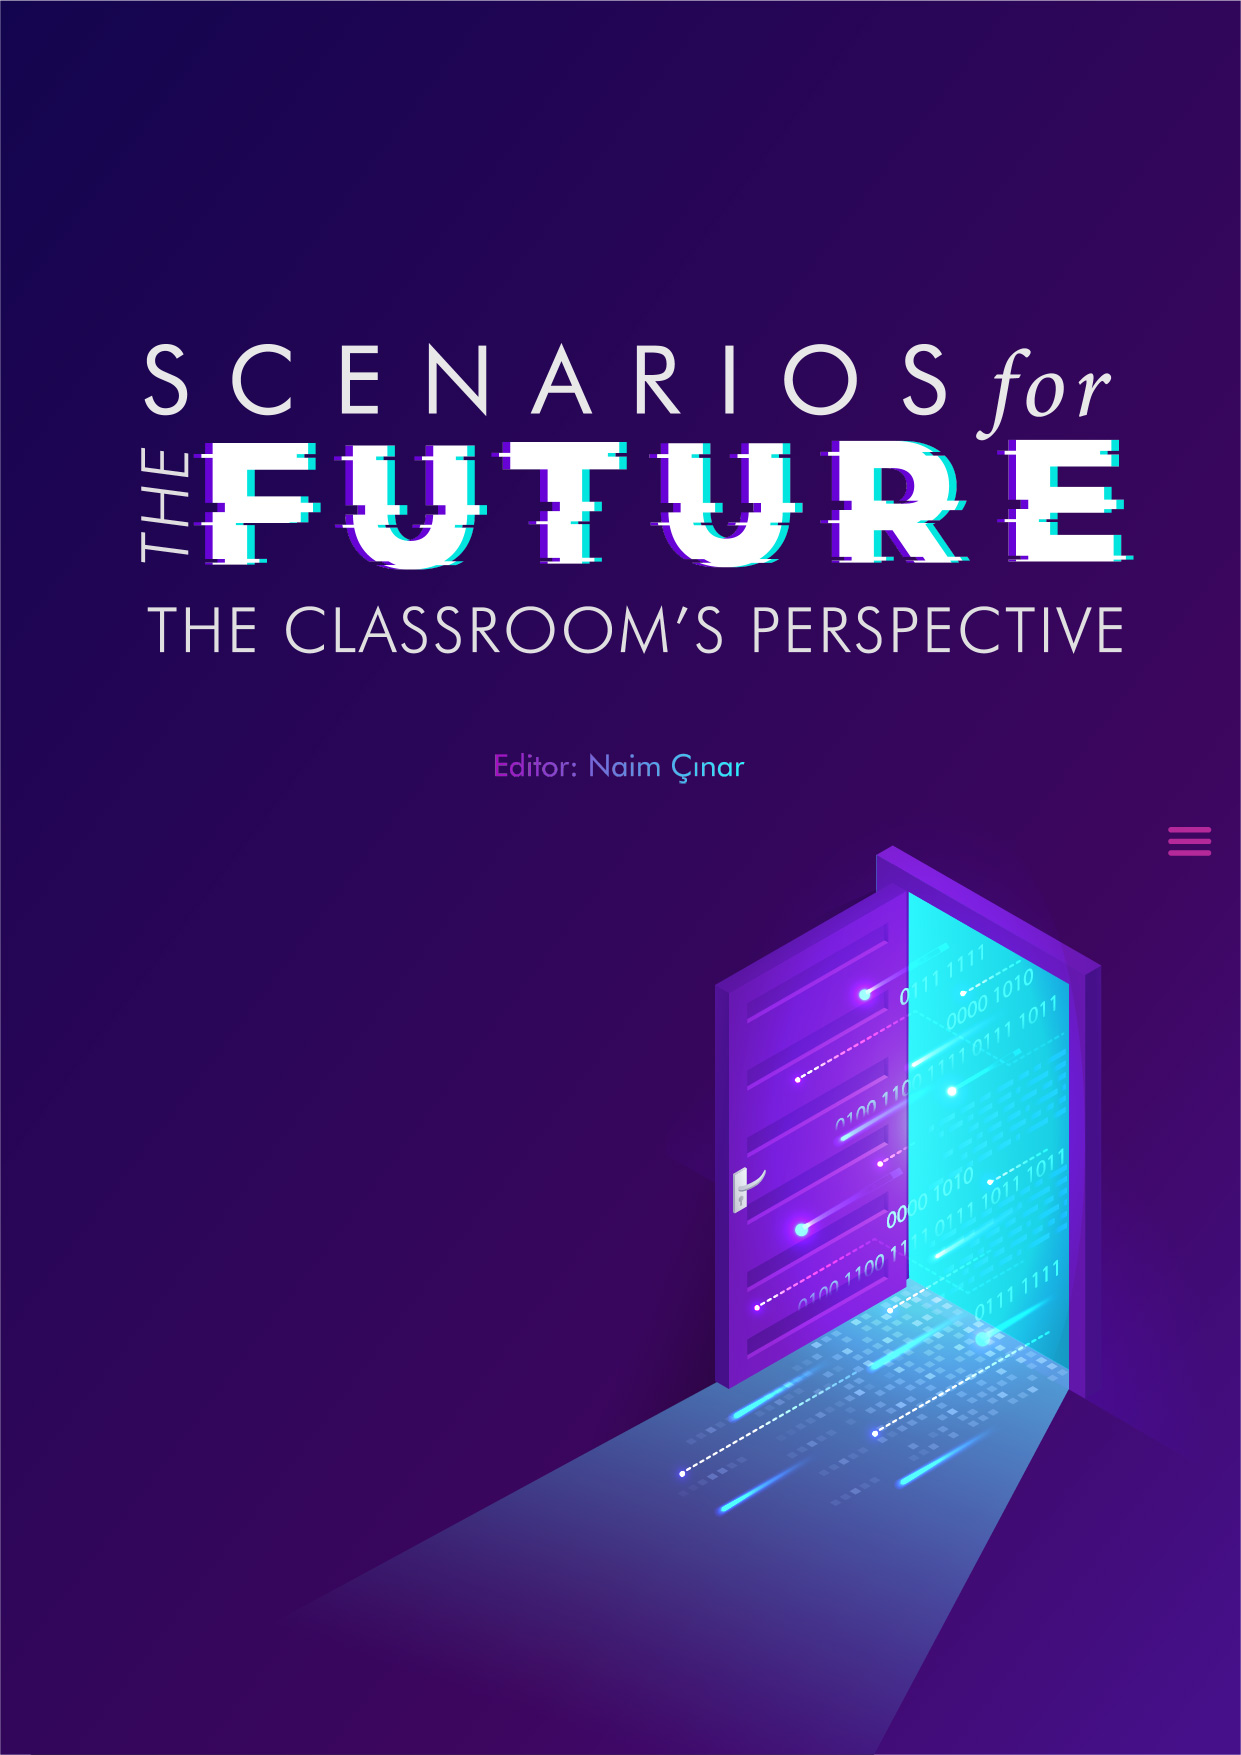
\includegraphics{images/book-cover.jpg}
Cover design: Berna Görgülü

This book was generated by Naim Çınar in \textbf{Markdown}, using R version 3.6.3

The \textbf{bookdown} package can be installed from CRAN or Github:

\begin{Shaded}
\begin{Highlighting}[]
\KeywordTok{install.packages}\NormalTok{(}\StringTok{"bookdown"}\NormalTok{)}
\CommentTok{# or the development version}
\CommentTok{# devtools::install_github("rstudio/bookdown")}
\end{Highlighting}
\end{Shaded}

This book is hosted on \textbf{\href{https://bookdown.org}{Bookdown}}

This work is licensed under a Creative Commons Attribution-NonCommercial-ShareAlike 4.0 International License.

\textbf{Citing the book}

As the structure of the book's chapters and sections may change, links should only use the base URL \url{https://bookdown.org/naimcinar/future-scenarios/}.

The full reference of this book is:

Çınar, N.(Ed.). (2021). Scenarios for the Future: The Classroom's Perspective (version 0.1.0, Feb 1, 2021).
Retrieved from \url{https://bookdown.org/naimcinar/future-scenarios/}.

\hypertarget{intro}{%
\chapter{Introduction}\label{intro}}

Later than the present time is always imaginary. We don't know the future but we anticipate it. Anticipation as here understood includes two mandatory components: a forward-looking attitude and the use of the former's result for action (Poli, 2017). The future does not actually exist. Therefore, hunting for futures run directly into the obstacle that by definition the future cannot exist in the present. And yet, the future plays a role in the present. How can something does not exist have an impact? An answer to this problem is the idea of anticipation. The future does not exist in the present but anticipation does. The form the future takes in the present is anticipation (Miller, 2017).

Anticipation is also vital for companies and organizations that want to develop convenient solutions to people's problems and expectations that might emerge in the future. To do this, the future consumer and technology trends are anticipated by doing extensive researches. Depending on these anticipations, some of the existing products/services are being updated or new products/services are being developed to respond to future needs of society.

I give an applied course called \textbf{RHI460 Advertising Project} at Anadolu University Faculty of Communication Sciences, and its content is based on the emerging consumer and technology trends. The aim of the course is to encourage students to think creatively about the future needs and expectations of the society. After an extensive analysis of emerging trends, each of them write scenarios for the future. Later on, they form groups and develop innovative ideas that might serve the needs and expectations of the future consumers.

This book, which is one of the outputs of the course, is co-created by the students. Each chapter is a future scenario that is based on a specific theme and a scenario archetype.

\textbf{Themes}

The major trends we have discussed in classroom-2020 are listed as: \emph{power of the crowd, individualization, urbanization, environmental issues, big data era, medical advances, offline experiences, play everywhere, betterment, connected, privacy concerns, disadvantaged groups, and security issues}

\textbf{Scenario Archetypes}

We used the six scenario archetypes framework of Fergnani \& Song (2020). In their article they list six archetypal images of the future, which are; \emph{Growthy \& Decay, Threats \& New Hopes, Wasteworlds, The Powers that Be, Disarray, and Inversion}.

I hope you enjoy reading these future scenarios written by young minds.

\emph{Naim Çınar}

\hypertarget{part-2020-21-semester}{%
\part*{2020-21 Semester}\label{part-2020-21-semester}}
\addcontentsline{toc}{part}{2020-21 Semester}

\hypertarget{section-id}{%
\chapter*{Authors List}\label{section-id}}
\addcontentsline{toc}{chapter}{Authors List}

The list of \emph{authors} who contributed in this section:

\begin{itemize}
\tightlist
\item
  Bahtiyar Eminoğlu
\item
  Başak Göksel
\item
  Bengisu Çelik
\item
  Caner Türkmen
\item
  Eda Şeker
\item
  Emre Taştan
\item
  Fırat Duğan
\item
  Hakan Hanay
\item
  Meliha İrem Ayvaz
\item
  Mualla Bengisu Demirkaya
\item
  Münevver Çelebi
\item
  Nazmiye Kılıç
\item
  Nihan Yıldırım
\item
  Öykü Tengiz
\item
  Sena Duran
\item
  Şerif Yıldırım
\item
  Sevil İleri
\item
  Tolgacan Sezer
\item
  Yağmur Ceylan
\item
  Zeynep Öykü Karagöz
\end{itemize}

\hypertarget{lost-in-galaxy}{%
\chapter{Lost in Galaxy}\label{lost-in-galaxy}}

by \emph{Bahtiyar Eminoğlu}

\textbf{Abstract}

\begin{quote}
\emph{Ramy is an everyday worker on the government. His job is to quality check a variety of products changed daily, inspecting them by the video stream of the security cams, but Ramy would start to get bored this underqualified job for him and start to quest the system. Newly developed technologies were not pleasing, and the feeling of long loneliness started him to be drawn into the galaxy.}
\end{quote}

``A hundred years,'' said the professor and waited a bit. ``A hundred years was the lifespan of an average human two centuries ago. Now, thanks to new AI management the average human lifespan is almost two hundred years, and two centuries ago human's biggest importance was their health. We are caring about your health, so you could go on\ldots{}'' Another workday starts with this unimportant boring AI propaganda, I just cannot listen anymore. I am constantly asking myself that ``What I'm doing?'' with my life, with my relations, and what will I do years later? If it is the same quality control bullshit, I will hang myself without a doubt. Probably those AI-integrated government drones would not let me even do that. I heard once that a man from Fonrade just thinks of killing himself and before he goes to his window the FRPD (Fonrade Robotic Police Department) raids his house and arrest him acting against the Pro-Life law. So, if my intentions get more intense any moment some Robo-polices could be up to my door. It is not living anymore, and you cannot be dear to die neither. The working screen is loaded. I am a current worker of the Governmental Quality Standards Institute. All I do is watching some CCTV of some companies and check if their product quality retains the government's expectations. The funny thing is, years ago a friend of mine told me that the companies send us some kinda video that was recorded years ago, again and again, just changing the dates. It gets funnier when you think more because if they send me the same video with different dates, I could not define if it is the same or different. When I think more about this, I am realizing that there is no window, no natural light source, it is indistinguishable from one to another. Today's company is a children's stationery manufacturer. Watching as the one blue eraser comes from the production line to the weighing and it is always at the same weight. A thousand eraser called as a party, and in every party, an eraser will select randomly and gets examined to see if it is having any hazardous elements that can harm children or having any defect or see the color of the eraser checks the company's standards. Subject \#986755 checks fine, subject \#987542 checks fine, subject \#989635 checks fine too\ldots{} I am getting bored as hell, but I am sure that like I control those erasers, someone was controlling me too. So, I am taking my notes and think different things to try to keep my mind safe. Subject \#990136 is fine, ``What should I eat today?'' Subject \#991247 is fine, ``What is on telly today?'' Subject \#992683 is fine, ``But I am not, though.'' Subject \#993548 is fine, ``why I am so alone?'' Subject \#994587 is fine, ``Maybe I was not fair to Jane.'' Subject \#995621 is fine, ``I wonder where she is now?'' Subject \#996852 is fine, ``Or what she is doing?'' Subject \#997159 is fine, ``Could we be together?'' Subject \#998020 is fine ``Why all the things happened this way?'' Subject \#999626 is fine, then an automatic message popped out ``Congratulations! Your work is done, for today. Thank you for your contributions to our community!'' \#Subject Ramy is not fine, \#Subject Ramy is confused, \#Subjesct Ramy is sad\ldots{}

I close my computer and get up from my chair. The computer said, ``AppleSoft Corp.~wishes you a good day, see you tomorrow!'' The only communication that I have for today was the two messages send me automatically from the server. I just lay down to my bed and open the telly, some stupid show was on. ``Microchips right, who is here loves microchips? It is something that helps our life I guess, but not on the planes apparently'' Everybody starts laughing, ``The flight attendant comes and says ``Sir, can you please shut down your microchips?'' And I just say, ``Wish I know how to do it?'' The usual situation, right? I wish the AI would find a solution to this. It will be like (In a robotic sound) ``I am the AI system bleep-bloop, you have no right to take a flight.'' Everybody laughs harder. ``Thank you! Thank You! I am Garry Samefeld and have a good evening everyone.'' Credits rolls and after that, there is a sponsor message, ``This show is sponsored by Laugh-AI, it will be hilarious with artificial intelligence when you are not so intelligent.'' Everybody still laughing and the show ends. Now the commercials start. ``Next week Human VS. Nature VS. AI: Who would win?'', ``The Treehouse Builders AI: Your favourite treehouse building show is back! And now with the new AI improved designs.'', ``Do you want a perfume that does everything you desire? Tell us your desires and we will make it happen with our newly developed AI system. Come to us, New Delphine AI Beauty inc.'' I really get bored with this stuff. I reach out to my Blu-Ray disc collection box. I found a disc that was a gift from Jane, we both love this movie ``On the Waterfront''. We watched this movie together maybe a dozen times, maybe more. New AI movies are not as real as these old movies. Scripts are awful, nobody cares about acting and there are no artistic directions. A stone-cold machine writes and directs 90\% of movies and series. All series become the same thing after all. The AI takes all the good bits from the old movies and breaks down to some little scenes, pastes all together, and makes a movie. Making all the parts good is not the same thing as making a good movie. They are just making some good clips and connecting them to make a monotone movie. It could be good for the people who cannot focus on the more complex things. They are easy to understand and people do not want to do the brainwork anymore. What a shame, there are no new movies that as half good as the good old ones. Jane was someone admiring this good stuff. I miss Jane, I should call her some time. When I watch the movie, I fall asleep. In the middle of the night, I hear some mechanic sounds, when I open my eyes a bit, I saw something passed in front of my window. Mechanic sounds said ``Ramy Johnson, we are arresting you due to your acts against Freedom of Speech Law and Government Pro-Life Laws. Please open up the door.'' I could not understand anything. After approximately ten seconds later an FRPD officer slam opened the door. They grab me from my bed and handcuffed me aggressively. I said ``What-what have I done?'', replied, ``Sir, you have the right to remain silent, we recommend you that.''. I was shocked could not do anything, I just said ``What have I done?''. The Robo-police answered, ``Sir, please do not resist the arrest.''. I could not get my thoughts together. I said, ``I am not doing anything illegal and I am not resisting, I just need an explanation for this situation.''. The Robo-police start to process and made a notification ``The suspect is resisting to the arrest, this is an attempt to prevent the justice system to function, the right act is execution the subject to prevent the malfunction! We will perform the execution to subject by firing each cop three shots at him, are you having any counter argument to the execution.''. I was blundered, I could not have my thoughts off from asking ``What I have done?'' to myself. In a spark of a moment I said, ``So it is an execution with fire squat as the only army force in the country are the police departments and there are more than one firing infantry.''. Robo-police asked me ``Yes, well what is your argument?''. I did not know what it will do but I asked to see if there are any chances ``Can I use my last cigarette right?''. Robo-police stumbled and said ``Well, yes but in our records, we clearly see that you are a non-smoker.''. I said, ``Well, I always wanted to try once, so can I get some\ldots{}''. Robo-police said, ``I do not have any smokes by any chance, but if you insist, we might have to go to the police center to give your last smoke and proceed the execution.'' I replied, ``Certainly, I do.''.

I was going in a police car driven by two Robo-polices. I was afraid and thinking about what I might do wrong, but I guess it was too late to think. I know watching old movies was not seem nice by the government, but it was not illegal too. Either way, now I was charging with malfunctioning the justice system and there is a death penalty on me. Maybe there would be a chance to talk to someone and cancel the death penalty. We were going ahead in a big way with high speed and I was afraid like a little child who runaway home. I stuttered and asked, ``Are you going to kill me?''. Robo-polices just laugh and laugh more, the Robo-police in the shotgun seat turned his head to me and prepared to say something, but an error occurred. First, the Robo-police's face screen twitched and turned into white and neon pink. Then it started to move randomly, there was steam coming from their body and both Robo-polices were frozen too. Slowly, the car started to slow down, I guess the driver was not stepping on the gas pedal anymore. There was a right turn ahead, but the car was going straight. I could not do anything, even the door was not opening. I hold my breath near the crash. All things are blackened, I open my eyes and saw the two Robo-polices was split into two. I slam my head to the driver's seat due to impact. I tried to open my door, it is opened, but I could not push the door, it was a bit jammed and I was in shock. I saw someone opening my door, a young lady with blonde hair. When she finally opens the door, I saw her face.
* Oh my god! It was Jane. Jane said ``Hey, Ramy did you miss me'' and grabbed my hand and pull me outside. I was shocked again. I was sitting on the side of the road and try to make sense. I said, ``H-How do you know I'm here?''. She said ``Listen when I break up with you, it was not anything with us, it is just something that I cannot tell you that time. I will explain everything, we just need to get away from here before more Robo-dummies come. She holds my hand and we started to run. I was not outside for years and we were outside the city too. Everything was different to me. We see some cops searching for us and the only direction we could go was a narrow street. We enter the street and keep running. A police van appeared behind us and it was coming fast. We were running, but not fast enough to run away from cops. The end of the street was near, but also impossible to reach without run over by the police van. The Police van was not going to slow down, they were not going to arrest us, they want to kill us. The end of the street was two or three steps ahead but still was impossible for us. Within my last move, I pushed Jane hard to the end of the street, but now the police van was running me down. It hit my shin and I fall really hard, I think I just broke my nose, the van was kept crushing my bones. The last hit comes to the back of my head. My skull is split open, the back of my skull snap and burst into the air and my brain was all over the van's bumper. Everywhere soaked in blood.

I opened my eyes, with fear, I was in my bed, I immediately look at my arms, they were okay. Then I touch the back of my skull, my skull was in one piece, my brain was inside, I was feeling okay. I heard a woman voice; Jane was sitting by my bed. I was surprised and said, ``Hello Jane, how all this happened?''. She replied with a formal tone ``Mr.~Johnson, the test that we had done yesterday shows us that you are completed your sentence and you are ready to come back in our society. We wish you luck in your next chance.'' And I said, ``Was everything here was fake?'', she replied ``In a way yes, but not as you think. All the jobs and tv shows, dinners, movies that you watch was a small reflection of our society.'' I was devastated ``But, I think we were\ldots{}'' she interrupted ``Lovers right, it is a basic misconception often prisoners make. They just want to make a connection with life, with someone and I am the only one that they saw in simulation besides robots. It is basic human anatomy. I will leave you now and let you gather your things, you have two hours to live, at the end of the two hours an officer will come and help with your departure procedure. Have a good day Mr.~Johnson.'' And she left.

I just do not know what to do now\ldots{}

\hypertarget{privacy-concerns}{%
\chapter{Privacy Concerns}\label{privacy-concerns}}

by \emph{Başak Göksel}

In 2070, technology is not the same as in 2020, but it was not that different. The screens we used in 2020 were still in our lives, but they were much thinner. After the crisis last year, people were afraid to live. In the past, there was nobody left who could look at those screens we loved so much for more than 15 seconds. Everyone in the world started to communicate with letters as if they were back in the past. With a total of 3 postmen left in the country - which is just for show - the most popular profession was postal business. I can hear what voices of the crisis that occurred last year. Although the crisis broke out last year, it has accumulated since 2032, but nobody knew about it. To summarize the incident, we have known for a long time that brands are listening to us over phones. But nobody was disturbed by this. As a result, what was artificial intelligence was the one who listened to us, what we were talking about as if it was important, they were listening and what was happening next, and it offered us an advertisement about it. When this is the case, the subject was closed when he did not care about the events in people. A new technology entered our lives in 2032. Small chip-like tools were placed under the skin of people with this technology. This chip-enabled us to project the phones we hold tangibly in our hands onto a surface or directly to the air as a projection. When the technology first came out, everyone was shocked. Because it did not enter our lives gradually like other technologies. For example, people did not get into electric cars directly. Hybrid vehicles were used first, then electric vehicles started to be used gradually and the environment reacted accordingly. But when this technology was launched, it was so affordable that there was nobody left who didn't use it. Using this technology in 2032 was equivalent to 4 breadcrumbs. Very suitable. We should have understood at that time that there was something wrong with this. However, we continued to use technology with pleasure for years to flow like water. Until 2057. This chip technology we used was supposed to constantly check people's health information and identify and warn possible diseases 1 week before. In 2057, most of the world's population consisted of elderly people. Coincidentally, most of the elderly, especially those over the age of 75, suddenly had a heart attack every day and hour. But since this is not news, people hear people who have a heart attack around them, but they did not know enough to spread it to the general, so they continued to give people their ages. I did that too. In 2065, the world population suddenly started to get younger. The old people died, yes, but the young people suddenly started to multiply. Even my friends who said that I never want children, the most important thing in my life is my career, had three or four children each. Everyone in the world was very productive and efficient. We were robots, but we didn't know. The years passed like this. A few people suspected what happened and tried to raise awareness, but no one believed them even once. They were in the same position as someone who says the world is flat in everyone's eyes. As the days passed and months passed, one of these suspects came out and spoke to people with a signal tone. Nobody understood what was happening, but everything he said made perfect sense. Because the sound of its signal deactivated the chips in our bodies for a while. He told people that they should get rid of the chips on their skin immediately. A few people with the courage immediately cut off their skins at home and removed their chips. Thus, the process of people's fear of technology started. People can be controlled, even sick and cured, thanks to these chips. We couldn't believe it. We lived in a huge lie. Who killed our loved ones? The brand that introduced this technology to the market\ldots{} Nobody was using the chips 2 months after these events happened. In this process, states took control and the processes of individuals getting rid of these chips were planned and they managed this process until there was no one left with a chip. Brand owners were sentenced to life imprisonment. But who would this punishment benefit? People stopped their phones and couldn't look at their televisions Those productive fertile people started living like plants. Because it was their success or what they did with the chip? People who could not find the answers to the questions started to get psychologically ill. Antidepressants have become unavailable. The world started to live like it was in the first ages. There was internet only in government offices and those who needed it could go and use it with an observer.

The effects of the crisis started to wane towards the end of the 2080s. People were a little more comfortable using Technology, but it was never the same. This situation affected natural states in every way. Most states have come to a tipping point. Later, all states gathered and planned how they could make people use technology. At this point where there is no trust in brands, returning was almost impossible for at least 10 years. In the states, they planned to change brands from private to state institutions. Since they cannot act according to their minds when they have a state at their head, individuals looked at this situation warmly. And all files of state institutions would be made public. Individuals would be able to access information stored about themselves and delete data they did not want. Although this solution doesn't sound very logical, the public liked it very much. Because the information these brands kept about them was disclosed to the people beforehand. People who read even the finest details about themselves allowed them to keep the information as they did in 2020. From being private to state institutions, brands gradually gained the trust of people for 20 years and gradually continued to privatize.

Nowadays, people are not afraid of technology as much as before, but they did not put them under their pillows as in the early days. But as time passed, people forgot what they had experienced, and people who had to go through this painful process got older. Including me. Now young people live with technology as in our early days. No matter how much it was told, because they didn't experience that fear, they could not grasp its seriousness. I don't know how it will be 30 years from now, but the situation does not look very bright. I hope the young people are careful and don't make the mistakes we made.

\hypertarget{growth-decay---privacy-concerns}{%
\chapter{Growth \& Decay - Privacy Concerns}\label{growth-decay---privacy-concerns}}

by \emph{Bengisu Çelik}

The year is 2040. Those who assumed that the capitalist system that had been going on for years would end were wrong. This system became stronger and the only power that could not be cut off. Covid-19, an epidemic of upper respiratory transmission that took over the world 20 years ago, was expected to keep everyone away from consumption and limit their socialization. But that's not the case. The Simple Life established at the beginning of the epidemic, celebrating the return of nature to itself, was a completely imaginary dimension.The system has renewed itself as much as it ever expected, and people have not given up on consumption. For this reason, the idea that capitalism had reached its saturation point was completely superstitious. The epidemic lasted for many years, suffering from various mutations.Humanity has dealt with various genetic diseases. Mental retardation was observed, especially in undeveloped countries and the elderly population was wiped out from the world. Generations hungry for consumption for years have left themselves in the arms of consumption, which they have blessed in the name of freedom.When the system reached its highest saturation, the existence of the state was now just a formality.

Big tech companies have once again realized how weak manpower is in the epidemic and have focusedof robots by eliminating manpower. That's why the economy was on the side of the strong. People were more and more faced with hunger and drought.The gap between classes, dating back 20 years, was now at its sharpest.He committed various crimes to maintain a lower-class life. Because of the water, people killed each other. Big companies have established dominance over people by using this situation as an excuse. Such great developments had been made in this direction that robots, the militar power of companies, responded to every resistance provided by states, especially those who refused to adapt to the new world order. Robots knew people by codes, and people didn't have identities. People had lost the concept of family. They didn't have names.

These robots were also owned by BostonDynamics, the company that had the most say in the world. BostonDynamics, an artificial intelligence and robotics design company, was founded in 1992 by Marc Raibert, a fellow of the American National Academy of Engineering, and other colleagues. Now the company is using States as intermediaries to carry out its plans and implementing what it has designed for the world without difficulty. The state went to food, electricity, water restrictions with the guidelines it received from the company. In addition, several other companies existed, and these companies used the underclass, which was ignored in the world, to add strength to their strength. Just as animal experiments were conducted for humanity in previous years, now the lower classes were subjected to experiments to further enrich the upper class. As those who succumbed to the epidemic, these segments lived outside the areas dictated by companies.There were no names of people here, and there were no names of days. The lower class was only allowed 6 hours of Sunday leave. It was also called Bostour. A combination of BostonDynamics and hour. Other days meant nothing to the lower class. In the same way, the seasons had disappeared due to global warming. Children living in great luxury in the powerful chain of the capitalist system, their robots told the seasons as if they were telling tales. Also most animal species no longer existed.

And the living spaces of those who held power were a completely different world. It was so fascinating that the lower class couldn't even dream of it. BostonDynamics branches allocated to our country by the United States took over places such as Istanbul, Izmir, Antalya. The winners of the system lived here in excellent city regulations and prosperity. Robots made the biggest contribution to this. Robots for all ages and identities were available. They were totally helping people. There was no transportation problem. Health problems were quickly solved thanks to medical robots. But for those outside the system, the situation was different. The robots were cruel to them. In experiments required by companies, these people were brought to the centers by robots.

For companies, robots could track these people's emotions and control their private lives. A separate unit called Robotic Sense Tracking and Response Team was created for these robots. Even if they acknowledged the cruelty of this, there was no other solution for this poor segment. They were bowing to the top. Otherwise, bad urban areas, the lack of hygiene of these areas were leading them to death. They were in need of help from the upper class. Exile was applied to the communities that made an attempt upon the re-strengthening of the state. People in exile were sent to places where drought prevailed, where earth resources were depleted, called the Emergency Traditional Fossil Fuel Accumulation Area.

When the stars of robot design companies did not shine so much, Microsoft complained of losing its throne, making itself known and once the richest in the world. He did not accept that such ruthless companies separated humanity with sharp boundaries. He was aware of the crimes against humanity and developed new software because he knew he could not defeat his opponents alone. He did this by first disabling robots responsible for sending people to be sent for exile, and training this audience under his own brand. It later blocked Bostondynamics' robots from accessing information that violated the privacy of lower classes. In this way, while the communities that made more revolts were sent for exile, they were actually fighters for Microsoft. In this way, Microsoft has at least managed to restrain the companies that are making the world cruel.

\hypertarget{landlessness}{%
\chapter{Landlessness}\label{landlessness}}

by \emph{Caner Türkmen}

\textbf{Abstract}

\begin{quote}
\emph{The natural balance of our world has been turned upside down. Natural disasters continued for years and all continents in the world except America were either shattered or swallowed by the oceans. A small number of people who have managed to survive in the world struggle to survive in the American continent.}
\end{quote}

The shelter, built to withstand all kinds of disasters, seemed to have worked. He had been lying left and right like a boat in the endless ocean for months. The supplies he thought would last for an estimated 6 months had decreased, indicating he had been in the shelter for more than 4 months. Again on such a day, he felt a strangeness, and he was hearing waves. The great excitement in him, this time when he put his head on the sunroof, he didn't want to see the ocean like a desert again. This time he wanted to see a piece of land. An amazing thing, if his ears were not playing tricks on him, he could hear human voices. He was afraid to leave his haven. People could be dangerous to him.

Imagine you are reading a novel, and the book begins like the paragraph above. You would probably think that someone survived the post-tsunami shelter, or that the sinking ship traveled in the ocean for 4-5 months with its specially made shelter and hit the shore of a region you thought was a primitive community. Or doomsday scenarios consist of phenomena such as thirst and meteorites. But I'm sure very few people would think the cause of this incident would be landlessness. I am also in that minority. For me, the end of the world will come from landlessness before thirst. Here, our hero was the conscious inhabitant of the land that was submerged months ago. Thousands of earthquakes have occurred in the world in recent years and these earthquakes have caused incredible destruction. Many continents are lost in the split oceans. All continents except Asia, Europe, Africa, and America are at the bottom of the ocean. Rising waters have absorbed a large part of the American continent. Earthquakes and streams of natural disasters devoured the mainland. Most of the people died. The lucky people who threw themselves into the American continent had to deal with insufficient resources. The world where the great utopia has been realized has been dominated by a single state. People also have no discrimination of religion, language, and race. Due to insufficient food and technology, people had to revert to primitive methods. It was understood that land was more important than money, and the state took control of the land just like money. The materials that could survive the occasional wreckage were worth wealth. Even though the vast majority of people perished, a considerable population was trapped in the American continent. People were settled all over the continent in a planned way. Thousands of immunocompromised people were dying here too. The crime rates had increased enormously and the state had become unable to control it. Criminals were sent to Alaska and left to die there. Those who were American citizens, whose personal and national interests prevailed here too, accepted that they were superior. They claimed that they should have a single voice in management. When these differences of thought caused conflicts in places, combined with the insufficient resource shortage, reactions and tendencies of violence grew and interventions became harder. All states in the American continent decided to unite and their center became Washington DC, the current capital of the USA. Each nation tended to colonize itself. Realizing this, the government made a planned distribution process and placed groups of different races in each region. Agriculture was completely under state control. Resource usage caused great controversy. Conflicts have already erupted in the south of the continent. People could not move even interstate without special passports and reason. Health and education were almost over. State authorities, who did not doubt that these conflicts would spread throughout the continent, found the measures to be more aggressive. The man continued to eat each other here as well. He used unimaginable resources to build weapons. The state is arming for the rebels, the rebels for the state. In such an environment, people had to live. Almost all electronic devices do not work. Satellite and wireless communications were over. People had difficulty even accessing electricity. Natural disasters for years have also affected the Americas. Everything turned upside down, and those that remained intact did not work properly. The state had virtually no technological material left. People exchanged by barter method. Mechanical tools for humans were worth more than silver, money, or even gold. The number of people looking for materials to explore and barter along the coast was enormous. The state could not find civil servants to employ. Because nobody cares about money. Only the state and people chosen by the state could produce a new product. Since resources were limited, the state wanted to control resource use.

In addition to all these, information was needed to improve the technology. Most of these sources of information had disappeared. The number of scientists was very small. State officials were still intending to search for a piece of land that had survived. The ships that remained in the hands of a few surviving states rotted from neglect, almost all of them became unusable. Natural disasters around the world left neither opportunities nor resources to care for them. As most of the natural disasters took place in the seas, marine vehicles were damaged the most. Government officials estimate that islands, large and small, may have survived in the most remote corners of the ocean. He wanted to reach them. To reach those islands, he was working on a ship project that could cross the oceans. This was a huge gamble. Most of the scarce resources and workforce would be spent on this project. The state aimed to employ criminals in projects for the shipyard and the state to provide labor. Not all was well for the people. Gangs that seized people's valuables had sprung up. They plan to own every valuable item during the exchange. They even used these materials to make weapons. Some groups were plunging into nearby areas that used to be living and now sunken in search of valuable items. The population was increasing steadily. But the only surviving continent was hardly enough for this population because living in a large part of the continent was almost impossible due to drought and desertification. People could no longer fit ashore. Water resources were almost nonexistent. The makeshift machines could not purify the seawater, people were getting sick and dying because of these water sources that could not be fully treated. Some of the scientists viewed this project as a waste of time and resources. He believed that instead of this project, it would be more logical to rehabilitate the deserts that cover almost the entire land. But the state did not take this into account. He was trying to reach the resources that would help technological development as soon as possible and return to the old days. People had a hard time finding food. There were a small number of living things that could adapt to the earth. Fortunately, although the fish population increased due to the lack of hunting, there were almost no tools and equipment to hunt them. Primitive fishing was done and sailing in makeshift boats. Although certain fish could keep up with this new world, it was not easy to hunt them. Fishermen were already going to take a great danger and go hunting. Gangs could easily kill people for fish. The state was having a hard time fighting the gangs. He could hardly prevent them. The state had already focused on the large ship project rather than preventing the turmoil. An act that is considered a crime in our daily life seemed like a normal act for those people. Social life had changed almost completely. It was not expected that people would attach importance to social life as the struggle for survival reached this point. 20 years from now, a newly born baby will not know what the object that hits the shore and what it does and will find the old world from a few pictures or some decaying books. Will things like books or pictures be so valuable that they can reach them? I guess, no. He would remember the old world only with the information that spread through word of mouth. Unless they were killed by gangs or lost his struggle to survive.

\hypertarget{overconsumption-and-then}{%
\chapter{Overconsumption, and then?}\label{overconsumption-and-then}}

by \emph{Eda Şeker}

\textbf{Abstract}

\begin{quote}
\emph{For a long time, we burdened our environment with our insatiable greed, we wasted precious resources, we kept asking for more and more, and we kept buying. At what price? Of our lives. Of our health. Our quality of life. Welcome to the year 2176, a world plagued by contaminated water, unbearable heat and crop failure, toxic air, and people with lost decency. In this world, where people long for the old days and are conscious of their guilt, there is a glimmer of hope during this apocalyptic situation. It is a curse and a blessing at the same time: the companies. Now it is their time to shine as the pioneer humankind needs and improve the critical situation with the latest smart technology. }
\end{quote}

The Secretary-General of the United Nations, Ban Ki-moon, once said: \emph{``We are the first generation to be able to end poverty and the last generation that can take steps to avoid the worst impacts of climate change. Future generations will judge us harshly if we fail to uphold our moral and historical responsibilities''}. If only everyone had such a determined attitude towards it. At that time, everyone had the same thought, at least hypocritically. Remember all those companies that made poor changes for the sake of their reputation and declared themselves eco-conscious? Remember the riled-up youth who marched on the streets every Friday to demonstrate against global warming? Well, this gave us the impression that we were capable of straightening everything out after all. It started promisingly, and it ended miserably. Soon the number of participants in the protests dropped rapidly. Schools forced their students not to miss classes. Businesses saw this as an opportunity to sit back and replay the old madness. As if that was not enough, they added to it: with constant enticements, such as reduced prices, they rushed people into a buying frenzy. Excess consumption blinded us, we knew that, and yet we gave in to it. The inner voice inside us took the upper hand, some would call it greed, but beast describes it better. Those companies knew what our guilty pleasure is and shamelessly exploited this. Eventually, they turned us into their greedy puppets. This marks the beginning of our catastrophe.

Imagine a world where the life we know, what we are used to, will not exist anymore. Now recall what your life is all about. Family, friends, school, university, your first job, colleagues, or your retirement? The daily routine you kept doing and following for a long time, be it for work or school. The surrounding you live in, the familiar faces, buildings, and maybe also landscape. Celebrating birthdays together, witnessing the changes in the seasons, or meeting with your friends in your favourite park. All of these are parts of our lives. Now imagine if everything that I counted before would be erased. Annihilated. Gone forever. Sounds terrifying, isn't it? Memories are the only things that remain. Can you picture living in a world, characterized by uncontrollable tornadoes, earthquakes, and unbearably long heatwaves? Where there are drought and crop failure, and people have lost their minds and ethics? Where each step outside equals a battle and matter of life and death? Think back to the dystopian television shows and series on Netflix that you have binge-watched in the past. They have become reality. You are a part of it. The world outside your door is unrecognizable. In some ways comparable to the Hunger Games but a thousand times worse. Any volunteers? Probably not, I would not want to exist in such a world either. Fact is we all do and just because we have no choice. Why? Because the long-feared global climate crisis had happened. We have failed. It is the year 2176. Decades of excess consumption and ignorance have resulted in our failure to approach the target set by the climate conference. Instead, companies have blown much more emissions into the air, and the use of synthetic materials such as plastics has increased sevenfold. I do not want to scare you off, but you should keep following in mind: Our air quality has deteriorated considerably. Greenhouse gases, such as methane, got into the air by the thawing of permafrost soils in the Arctic and Siberia. Without special breathing masks, it is no longer possible to get outside. Because of the carbon dioxide in the air, the sky is brown. Just from looking outside, you realize how polluted it is. It is much worse than the smog images you have seen on the news from China or India. When going outside, you need a flashlight to not get lost. It has become rare that you see a human being leaving his or her house in times like these. But when people dare, it is only the brave ones. Stepping out the front door seals your race against the polluted air, the stifling heat, the sea of plastic and people who have lost their minds. Pretty apocalyptic, don't you think? You cannot recognize our environment anymore; the consequences of climate change have hit it hardest. Our ecosystems, habitats for numerous species, are defenceless against the scale of global warming.

First came the heat. Suddenly, the entire globe became hot, not warm, but boiling. 52 degrees Celsius. Nobody remembers snow anymore, because the only season is summer. You can probably guess what a disastrous chain reaction this set off. First, people hoarded entire water bottles in supermarkets- when they did not care about the heat. With the heat, water consumption increased sharply, because everyone stayed at home or in places that gave them shade. Within a few days, the water shortage came. Governments tried to call people back to their senses and pull themselves together, but everyone had better things to worry about. At the same time, the permafrost soils in the north melted. As this appeared in the news, the entire human race broke into a panic. The governments of the countries ordered everyone to stay in their homes. In a short time, all the stores closed, and public life died. This marks the beginning of the darkest chapter humanity has ever seen. No one had protective clothing or masks against the toxic greenhouse gases. Militaries distributed - strongly reminiscent of the times of the World War - emergency packages, which they threw down from the airplane to the towns and villages. If you were lucky enough to get one and not be attacked by civilians running wild, you received a special protective suit with a matching breathing mask. Gone was human dignity, respect, or compassion. Instead, it was about their survival. No one had any regard for their fellow beings anymore. It is one against all. Unfortunately, many animals suffered a lot from the heat. Without water, they had no food and nothing to drink. Soon, we became witnesses of the first extinction of some species. Large mammals, such as elephants, giraffes, or zebras extinct. But it also affected the carnivores, reptiles, and amphibians - they all had no chance. Countries alongside the equator have become uninhabitable. India, Bangladesh, or Brazil resembles extinct deserts. Millions of people fled from their countries either south- or northwards. No one would have thought that our environment would be our undoing. You must be wondering who goes out at all in such dire circumstances as these. Well, we all need sustenance, remember?
Speaking of food, this is the second big issue we are dealing with. Logistics can no longer provide people with everything given the circumstances. The loss of food and hygiene supplies hit us very hard. People realized how many of the products they were constantly consuming were imports from all over the world. For people in Europe, for example, this meant no more fruit from the subtropics and no more rice from Asia. Instead, they began to scavenge in the fields of local farmers. The last time Europeans could eat rice or mangoes was decades ago. But because of the heat, agriculture was plagued by crop failure. Poor harvests everywhere were the result of an unbalanced diet and a significant vitamin deficiency. Soon we were struggling not only with the heat and the gases but also with our bodies. A lack of hygiene products also meant that we became ill more quickly. Our immune system was deteriorating rapidly. We had never been so weak and exhausted. Here it became clear who was the strongest: the poor and homeless, who had neither money nor shelter, suffered the most. They were the first to die just like new-born babies. Politicians spoke of a ``human crisis'' whose extent resembled collateral damage. We thought it could not get any worse than it is now. But we were wrong.

Instead of trees and flowers, we have vast amounts of plastic of every kind. Plastic bottles, car tires, fishing nets, plastic packaging and much more. Plants no longer exist because of the drought and lack of water. The plastic we have consumed and threw away in the oceans and ground got washed up to our doorstep because of the rising sea level. Waste disposal companies are overwhelmed and can not cope with the gigantic amount. The world has become one large wasteland. Another threat arising is that the glaciers on the Arctic have melted and, thus, the sea level has risen significantly. As a result, floods threaten many African countries. Madagascar, for example, turned into the second Atlantis. It vanished within a few days after the sea level rose. Besides, West Europe is also underwater: Netherlands and Belgium do no longer exist anymore. Many no longer perform their work. Of course, who would want to work anyway? Unfortunately, many shamelessly exploit our plight and demand a high food price. People quickly ran out of money. As a result, vigilante justice and serious fights happen daily. They are hoarding leftover food everywhere. Our everyday life has nothing to do with order and decency, people have become like beasts. But it is not just citizens who are going through a metamorphosis, companies are too. Everywhere, they declared bankruptcy and shut down their production facilities and factories which explains why logistics cannot conduct their business. Till now, there is still is a lack of raw materials, natural and physical resources, and water- everything we do not possess at the moment. A real disaster.
The question that remains is: who is to blame for everything? Who is responsible for the never-ending suffering? Who is responsible for the natural catastrophe? Who is responsible for the several deaths of individuals worldwide? Let me guess you would instantly point at the companies. Am I right? But have you thought about who contributed significantly to this as well? You. You as in every citizen, ordinary people, neighbours, colleagues- every single person on this planet. The answer to everything is everyone. Every single one of us has been either selfish and ignorant or stubborn. Admit it you count to those people as well. We all do. In times before this madness started, we wanted everything at the cheapest price. As long as it satisfied our insatiable needs and gave us prestige, we were happy. We did not care about the materials, the environment or whether what we were buying was actually of any use to us. The attitude of each individual to neglect the global problem and maintain the same consumer behaviour has ensured that we have to bear the terrible consequences. The old, happy, and carefree life is history. Our reality is horrifying. In the past, the more, the better was the rule: The newest technologies, latest trends in fashion and lifestyle, better telecommunications. Fear of missing out (FOMO) was driving us insane, making us order too much online, shop until we had no money left in our bank accounts, and get lost in all the excessive products. Influencers on social media and celebrities amplified this wave. Our situation is very similar to the apocalyptic blockbusters we used to watch and enjoy in times of consumerism, which made us underestimate everything. We are now witnessing real-time cinematic experiences. Society got divided into groups called clans. All clans have the same goal: to occupy a valuable source (a water source, fruit, or oil) and to deny others access to it. Robberies, violent confrontations, and killings are daily occurrences. No one takes responsibility for their crimes; everyone has more important concerns. A hundred years ago nobody would have believed that we would fall so deep. You are probably asking yourself how it is possible to survive in this world. Ironically, it is due to many companies. This global warming crisis has slapped everyone hardly. The majority has -finally- noticed that we are in the last stage. Excuses and blaming others are no longer valid. Everyone is responsible because we are all inhabitants of this planet. We were used to trusting that someone else will save us. But this thinking has led us to this situation. Everyone believed this way, and nobody acted. Regret and sorrow fill us all. Only now do we realize what a great opportunity we had, and yet we had not taken advantage of it. Time has punished us. From now on, things can and must get better; the proofs are screaming for it. What we should have done a hundred years ago, the future generation is doing with its own hands and strength. Sustainability, recycling, and careful use of scarce resources are the crucial points of their actions. However, they must give back what they have taken away from nature. But many of us do not possess needed equipment or have a lack of expertise. That is where the companies come into play. They are not only pioneers of a selfish population, but they also teach us, open our eyes, and show us what our behaviour has led. But who are they?
Behind all these global brands are scientists, academics, and entrepreneurs who took our terrible problems to heart. When the first announcement from them came on the news, hope sprouted in us for the first time. Hope that we thought we would never feel again. The companies were aware of the great burden on their shoulders, the great challenge that lay ahead of them. Everyone had great expectations of them. They knew it will be hard, but they also knew that shying back and giving up was not an option. Billions of lives relied on them.

In strong cooperation among themselves, they worked and experimented at high pressure on innovative solutions under limited conditions and came up with an impressive collection of inventions within a few months. Now, everyone works together and not against each other because we are all in this together. They say necessity is the mother of invention. Within a few weeks, they developed new concepts and invented a series of new products. One of the most effective and important inventions are emission vacuums. As the name says, they are soaking up all the carbon dioxides and methane in the air. Smart technology enables that this input it soaks in is transformed into renewable resources as the output. Thus, metal is the product you win. The prototype has been tested in the region where pollution is the worst: South Asia. India and China, especially, had vast amounts of gases which left them in darkness. After two weeks, the air quality has improved significantly. The people were amazed and released at the same time. Afterwards, several emission vacuums were distributed on the continents with the help of militaries. Their distribution was difficult and took a while since transport systems are still out of service and the scarce fuel reserves. However, it did not take long until we could see the sun, which plagues us with heat, again. But this time we were grateful for it. Another big change happened in the cities: the latest technology in genetic research has made it possible to artificially breed crops and other foods. They require less to no water at all and are resistant to environmental influences such as heat or toxins in the air. This saved many farmers their harvests because they could plant five times as many fruits and vegetables, cotton, or grain with the given area of plantations. By using drip technique, which countries in Saudi Arabia have been using for a long time, we ensure sustainable water management. Besides, cities started to take more shape: Trees and shrubs protrude from every building's façade. Thus, it is not only contributing to better air quality but also giving birds and other small animals a new habitat. Scientists have proved that with the use of especial pots, trees survive in hot climates like deserts. They are from recycled paper, combined with a specific soil mix they can grow in the heat without new water intake for weeks. Africans and South Asians are lucky since they can harvest fruits and nuts in their regions as well.
There is one invention I am very pleased about: against the long-despised plastic, scientists found a sustainable substitute: sugar cane. Every bottle is made from this and is biodegradable; we no longer have to worry about scenarios like the plastic floods in front of our doors. Another essential change is the way we treat goods. As you remember, we used to throw things away when they were broken, damaged or not working anymore. Ever since the changes arise, we realised we avoid excess and waste disposal by thrifting or letting our items fixed. Thus, small businesses were able to open again and flourish. Especially for electronic devices, whose recycling is complicated, this solution is very effective. Every little component of a product is reused, which means that no new items are required. The same applies to textiles. Fashion, which we adored a lot and was our guilty pleasure, is different from what it used to be. No one purchases new clothes; we thrift and exchange instead. Big clothing companies had to close forever. They realised that their business model is not suitable and can not coexist with the different mindset of ours.

What remains is the heat, it is unbearable as before, but scientists have also found a solution for it. Special solar cells reflect the sun rays and, thus, the heat as well. The construction of these plants took a very long time, after all, everyone in the world suffered from it. Years passed. Eventually, our long wait was rewarded with pleasant 28 degrees Celsius. Do you see what wonders companies worked? Let me remind you they are the same who fed us with their ubiquitous promotions and inducements until we were sick of it. It is remarkable how a crisis changes both our mind and society. From now on, a chain reaction of social awareness started. After we could breathe freely without protective clothing and masks, and the heat could not harm us, we began to engage in activities. Every one of us started to socially participate, be it looking after the poor and homeless people, cleaning up the neighbourhoods, or supporting farmers with their harvest. We became conscious citizens.

Humanity has come a long way. We have been through the worst, endured a lot, but we are coming out braver as ever. Looking back at the past 12 years of this change we learned a lot during this transformation. In these 12 years, we have lost 2,678,492 people, 65,345,788 species, and thousands of hectares of precious ecosystems. Accepting these facts is hard. We have lost a lot. Unfortunately, we cannot compensate for a lot of things, the damage was too severe. But that does not mean we can not improve and protect what we have now. And this is the course we are taking and aiming for.
None of this would have been possible if pioneers had approached this problem with ambition and will. It is inconceivable that our ignorance and laziness led to this disaster when all it demanded was discipline and dedication. We alone are responsible for this earth, because if not us, then who? We could all have prevented this if we had worked together. Without global brands, the world would probably have been so contaminated and polluted that everyone would have died immediately. Maybe none of us would be alive. Our behaviour and attitude towards the environment have changed significantly. Gone are the consumers; we are all conscious people. We no longer buy to enjoy. We create to live better by showing our respect for nature and giving back to nature what we take from it. This balance did not exist in the 21st century. It is a big lesson for all of us, which we will not forget easily. The global crisis has shown how frightening it is when Mother Nature strikes back. It will take time to reach this balance, how long nobody can estimate. A few months, ten more years, or several decades. What counts is that we are finally moving in the right direction and that we can secure the future. Our future generation will thank us for this necessary and considerable change. Regardless of what comes, we will ensure that future generations will have a forthcoming because we will pass on to them the precious treasures of this planet. Until then, we will continue, and we hope so will the generations to come.

\hypertarget{message-from-future-to-future}{%
\chapter{Message from Future to Future}\label{message-from-future-to-future}}

by \emph{Emre Taştan}

The YEAR 2040 \ldots{}

I'm 100 years old today. Considering that the average age of death is 120, I have 20 years left. I've seen many eras since 1940. I've experienced them all. Before I died, I wanted to convey this change to 2060. There are big differences between the periods when I was born when I turned 50 and when I turned 100\ldots{} Technology has changed people in every field. Some of these are;

Small-scale personalized production is dominant rather than mass production.

Physical brands have largely lost their importance \ldots{}

There is a race to grab space for hologram advertising in the sky \ldots{}

Ads are everywhere thanks to digital lenses. These lenses record everything we look at and advertise things we might be related to by matching.

High school goes on and on. Let's get into the details.

Technology is a phenomenon that develops, changes, and renews people. Although technology and people were out of step in some areas, this offered them new development opportunities. For example, with the help of technology and robots, humans have largely been out of action for jobs that require physical strength or analytical intelligence. Because robots and new devices can do these tasks hundreds and times faster and more accurately than humans. At this point, people become inefficient. But this leads people to orient themselves in new areas and acquire new skills. Because the definition of JOB has changed.

BUSINESS = CREATIVITY

Technology and things that robots cannot or can only partially do - that is, creative work - have become people's new focus. The symbol of success and being equipped is now ``creativity''. People who can bring their creativity to the forefront in their work are becoming more sought after.

Of course, creativity is not the only thing needed. Another important factor is specialization. To be able to do more professional work and to solve the unemployment problem, even for small jobs, specialization was made. So people don't go to the same person for the digital lens and the digital ring they have problems with. He goes separately to the digital lens specialist for the digital lens and the digital ring specialist for the digital ring. This approach promotes development as it leads people to specialize in specific fields. Besides, it prevents unemployment that can be brought by the increasing population with a wide range of jobs.

The change in the job description and the increasing importance of creativity and expertise also affected the education provided in schools.

In a world where technology and creativity are the main elements, the education given in schools has focused on specialization, technology, and creativity to meet the needs and provide the necessary human development. People receive training in very specific fields, develop themselves on creativity, learn techniques to use in business life, and meet their daily needs. Individuals who cannot use technology are not considered to be in this world.

Another important point in education is; training takes place in a physical environment. Although the school focuses on skills such as creativity and specialization, it has a very important output: Social skill.

The fact that people have strong ties with technology causes this technology to create a world within the person and to be isolated from people. For this reason, people's relationships with other people have weakened so much, and he forgot to communicate with each other ``like a human''. With the agreements made between governments under the leadership of Harvard, schools have been transformed from virtual environment to physical environment, considering that it is a suitable environment for people to develop these skills.

Many objects have emerged that people have to carry in their daily life. People have more than 10 internet-connected devices. These devices are not a pleasure, but a part of people's lives. All of them are elements that improve and facilitate people's lives.

Digital lenses, the most widely used wearable technology product by humans. With the increase in vision problems due to technology, Google came to the rescue of people and introduced ``Digital Lenses'' to people. These lenses have a clearer vision than a normal human eye, as well as a device that can be connected to the internet. This is the most important point. Since the device is connected to the internet, everything we can do over the internet is right in front of our eyes; calls, messages, even people's information.

Many brands have produced software for these lenses. The most effective of these was Facebook. Thanks to the software that Facebook makes to the digital lens, the profile of the desired person can be seen when looking at that person. Thus, the desired person can be contacted easily. We no longer need to go ask or search for hours to find out someone's name, age, or profession. The only thing to do is to look at the person whose information we want to learn and access their information.

Also, ``Electrıcfoxy'', which has taken the opportunity of many people to use digital lenses, started to produce digital clothes suitable for these lenses. Thanks to the chip placed on the body, the person can easily catch the fashion without effort. You load the purchased clothing models into the chip and wear them whenever you want and change them whenever you want. Thanks to its personalization, its size, size, and color are made as desired. Now we can say that fashion is at our fingertips.

Technology and these devices have helped people have more say about their health. So it is more dominant on people's health. Thanks to the ``Digital Ring'' produced by Apple, it displays harmful cells, muscles, tissues, tendons as well as simple measurements such as sugar and blood pressure. All you have to do is hold it over the desired area and look at the results from the hologram.

Besides, the ring can be used not only for health purposes but also for communication. Thanks to the hologram image, it includes operations such as speaking, searching by voice command, and navigating. Thus, a small tool has increased people's control over themselves and made it easier for them to communicate.

With the increase of robots, people's sports habits have also changed. Robots specific to each branch are now available. People buy these robots, customize them, train them, and put them into competitions. For example, consider a boxing match. Robots come into the ring. Each robot has sensors attached to the robot on its owner. Thanks to these sensors, whatever movement the owner of the robot makes, the robot instantly makes this movement. Thus, robots fight through their owners. Of course, this applies to other branches as well. In athletics, robots own effort, but the runners are robots.

Even sports have changed, but the subject of food has not. Eating is a pleasure for humans. One of those rare things they won't give up. For this reason, the subject of food is the same as in the past. But there have been changes in the way of production. In order not to accelerate the bad course of nature, the animals (especially meat-producing) were extinct. Under the leadership of Impossible Foods, meat production in the laboratory has reached 100\%. It's not just meat. Many products are produced in the laboratory. Cheaper, more nutritious, tastier, and more environmentally friendly.

The increase in the human population and the filling of the lands made transportation difficult by large vehicles. For this reason, electric autonomous bicycles have gained value and have even been made mandatory in many places. With the autonomous electric bike made by Xiaomi, people have entered a comfortable, fast, and space-free era in transportation. These bicycles, which are quite fast, are compatible with smart roads, take up little space and have a zero accident rate.

Finally, I want to list a few more things like at the beginning;

People are very lonely in their daily life. Because they have a virtual universe of their own. For this reason, they spend most of their time at home. Thanks to enhanced technology and wearable technology, she enters the virtual world - games - and engages in activities, and lives in the world she fictionalizes and desires.

Many small things it needs can be easily produced in seconds with the 3D printer in their home.

People are not cleaned with water. The approaching water shortage kept people away from cleaning with water. Brands led by Unilever have introduced shampoo and cleaning products that do not need water.

I hope all this 2040 information will move to the year 2060 and let them know about their past.

\hypertarget{tap-to-reset}{%
\chapter{Tap to Reset}\label{tap-to-reset}}

by \emph{Fırat Duğan}

\textbf{Abstract}

\begin{quote}
\emph{Jason L. is a cyber-detective. His mission is the catching the cyberbullies. However, Jason got a case one day. The man whose name is `There\_is\_no one' is in the police department and, he had some information about a big cyberbully.}
\end{quote}

\textbf{Everything Started with a Coffee}

Jason L. was a outstanding cyber-detective. He was not a big person that all. He didn't have big biceps but, he was really good to use computers and cyber systems. He hacked Google servers in 12.5 minutes during his junior years at the police college. He was nearly kicked at the school but, the professors didn't allow him to. After his graduation, he got lots of cases and, he got a promotion really fast.

He came to the police department. He tried to remember what he forgot. However, The office chef Melissa called out to him when Jason got to his chair. She had a case file in her hand that was a big title on its top.

Jason went to Melissa's room and, he closed the door. Melissa looked nervous. `What is the problem?' said Jason. She gave the file to him. Jason's eyes got bigger when he read the title. The title was `There\_Is\_No\_One'. Jason remembered what he forgot suddenly. `I need a coffee!' he said.

\textbf{The Lockdown}

Judy L. Harris was a good citizen and, she was an honest gynecologist at the Millennium Hospital. She paid her taxes, fallowed the rules. There was not even a parking ticket.

She woke up and started getting ready. `Alexa, play Rossini, please!' said Judy. She opened her laptop and checked her mailbox. There was an e-mail regarding the new hospital rules. She didn't realize her laptop was hacked by someone when she clicked the mail. The music stopped and protection cages landed on all the windows.' You are a cyberbully. The police are coming. Stay calm and, wait. You will not be harmed if you cooperate. You are on lockdown.' said Alexa.

\textbf{There Is No One}

Jason knew that nickname. That nickname was a sign who belonged to the hacker. `Where is he now?' he said. `In the interrogation room.' Melissa said. Jason tried to go to the interrogation room very fast but, Melissa stopped him. `He came to us voluntarily. He wants protection. In return, he will tell us everything she knows.' Jason was surprised but he didn't show her. Before exiting the door, he turned and said `So give him to it.'

There was a woman on the chair in the interrogation room. Colored eyes, blue hairs\ldots{} She was nice. When Jason entered the room she looked at him. `Oh! Famous detective Mr.~Jason L. How are you today sir?' she said. Jason sat on the chair and, drank his fresh coffee. He said `You already know me. I will not introduce myself but, who are you?'. She leaned forward slightly from her chair and smiled, taped the header on the file twice with her finger. `Mr.~L. There is no one. You are not talking to somebody right now. I'm an unidentified person. Whatever. The real question is why am I to here?' Jason didn't say anything. 'There will be a heist. They will steal people's IDs. Newborn, child, adults\ldots{} Lots of ID. All the persons who have a file at Millennium Hospital in danger.

`How do you know that?' Jason said. The woman sitting in the interrogation chair leaned back and said `I wrote the software for stealing the IDs. Stanley Jacobo gave orders.' Jacob was shocked. `Stanley Jacabo? Owner of the Millennium hospital and future presidential candidate? But why?' he said. `Info is the power.' said her and, continued `If you want to catch him you need someone inside the hospital.'. Jason looked her eyes and ask`Who and, why?'. The woman smiled and said `Why? Because someone has to go unnoticed into the ID registration room and insert the flash drive into the computer. That person is Judy L. Harris. Don't worry I brought her here for you.

Detective Jason entered the room that Judy Harris is held. Doctor Judy looked at him in panic and said `I did nothing officer. I swear.' Jason said her `Calm down, Mrs.~Harris. Are you a doctor at Millenium hospital?' Judy nodded in surprise. `We need your help.' said Jason.

\textbf{Co-oparation}

The next day, to begin her work, Doctor Harrison got out of her car in the hospital parking lot. She passed security, smiled at her colleagues. After getting on the elevator she heard a voice inside her ear. `Nice! Stay calm and keep moving.' said Jason. Doctor Harrison said `Ok!' and, after getting off the elevator, she headed straight for the registration room. When she was going to have the pass card read, someone called her.

`Mrs.~Harris! I am looking for you. We need to talk. Let's get my room.' said the manager Lawking. She walked with him to the room. She was nervous. The manager asked `How was your yesterday Mrs.~Harrison?'. `After hard work, some vacation was good.' she said. Judy heard Jason's sound in her ear again and he said `The manager is suspecting something. Tell him a lie.'. Doctor Judy continued `I watched film and got rest.'.

The manager was not interested in what she said. He took a sheet of paper from her desk drawer and held it toward her. `Here's everything you need to quit your job, Mrs.~Harris. You can tidy up your table. Thank you for your services.' he said. Judy shocked. `Sorry. What?' she said. `You've been fired. You can out. Thank you.' said the manager in a cold voice.

Jason and Melissa looked at each other in the secret trailer outside. Judy desperately left the hospital and walked towards her car. `The whole mission has been ruined, what do we do now?' Melissa said. When Jason turned to reply to Melissa, a black panel van appeared on hidden cameras. The van went near to Judy's car and the back doors openned. Two men caught Judy and took the van and dissapered. It was too late when Jason and Melissa realize that.

\textbf{Back to the Batcave}

Jason burst into the interrogation room. He shouted `What have you done? You know they are watching.' The hacker said `Yes, I know. Because of that, I gave you the flash disc. It was a GPS. I can find where she is and, I can shot down the software before the heist. Jason was angry. He said `I don't trust you!' She said `You don't have another chance. I need my computer.' Jason thought and `We can arrange a computer for you.' She said ` No, I need my computer.'

After Jason set the required permissions, they went to the house of the hacker with Melissa. That house was a regular apartment. There was not an extreme thing. House decorated was relax. There was not too much furniture. When they entered the hacker's working room, they saw a computer desk but there was not a computer case. All the desk was designed with computer parts. Jason looked and said `Oh! Fascinating. Do you steal IDs on this computer, don't you?' The hacker just looked at him and smiled.

After a half-hour, she said `I found her.' Jason said `OK! I will call for support. The hacker said `Calm down, boss! She is on the depot where the server has the software. If we are caught by them they kill all the clues and girl.' `Can you shut the server down?' said Jason. `Yes but, I need to access the server manually.' the hacker said. Jason looked at Melissa and, Melissa call the her assistant.

\textbf{Who Are You?}

Judy was scared so much. Who were these guys and, why they chose her? Then, she heard a man's voice. She knew that but, she couldn't remember. Who was him? They pulled out the sack on her head. She saw the manager Lawking at the Millenium Hospital. The manager said `How was your day Mrs.~Harris.' Judy felt like she fell over the cliff. `Do you know how are IDs cost on the black market? Why everyone should has just one account on the pc? It's sucks. I give them their freedoms. I will burn this shit system. I will burn this shit system. After that, I will say Stanley Jacobo did everything. I will be rich. Jacobo defends this system because he wants to be a president. I worked at that hospital for years. What did he do for me? Nothing. I will burn him too.'

To the outside, the special forces surrounded the areas. Everyone was ready for the order. Then Jason said `Now!' on the radio. When the manager Lawking heard the gun voices he started to run to the back door. However, Jason and his team was waiting for him. They caught him in easily.

Jason took the hacker and run to the depot. Judy was tied in a chair and was not moving. She fainted with fear. They untied her and Jason went over the radio for the paramedics to arrive. Melissa came to them really fast and said to Jason `Take her and, go to the server. We will be here.'

The hacker went to the server with Jason and, she took every clue for cops. Then shut the software down. When Jason took the hard disc that has the evidence he looked at her and asked `Really! Who are you Mrs.~There\_is\_no\_one.'

She laughed and said ' I am the hacker and also I am the daughter of the owner of the Millennium hospital.' Jason was shocked. `My father and I are not meeting, but I knew he wouldn't do such a thing. my father is trying to prevent people from living what they went through before the great cyber-war. I support him and this system.' Jason was shocked again. He started to laugh and said ' You are a hacker and you support this system?' She said `Yes and I am an detective too. I'm Melissa's mole inside. We have been conducting the operation in secret for years. That's why you've seen my name in so many places.' Jason looked her and said `Your nickname!'. The hacker said `Oh, yes. By the way I am Sarah. Sarah Jacobo.'

\textbf{Everything Is Fine}

After the operation Jason, Sarah and Melissa went to the hospital that Judy was being treated. She was fine. When they were talking to each other Stanley Jocobo is came to the room. He said `Hi! I hope you are fine.' Judy was not expecting to see him. `Yes, I am. Thank you for your visiting.' she said. `Oh! Don't thank me. If our professional cyber-cops didn't catch them they could do many worst things. Moreover, it is my duty to visit the new director of my hospital.' he said.

Judy was frozen. `Th\ldots{} Thank you!' she could say. `I hope you will be fine as possible as fast. We need you.' he said and he smiled her. He turned to Sarah just as he was going out, and said `Maybe you'll come to dinner on the weekend. Your mom will cook your favorite food.' Everyone looked at the Sarah. She could not hide her smile and shook her head positively.

After telling Judy to get well soon, Melissa left them. Jason couldn't stand and asked Sarah `Why you don't talk with your father?' She looked him and said `I will tell but, I need to eat something.' Jason looked her and said `Yeah! I need coffee too.'

\hypertarget{the-crow}{%
\chapter{The Crow}\label{the-crow}}

by \emph{Hakan Hanay}

\textbf{Abstract}

\begin{quote}
\emph{After the migration, earthlings were busy with the Techno Helmets in Alpha Centauri.}
\end{quote}

When humanity completed its migration to Alpha Centauri, they said goodbye to each other and settled in the one-room, high-rise buildings called Technopolis. Technopolises were areas designed only for one person, where the control was easy and people could not communicate with each other. Centaurians were able to get food and drink from vending machines only on certain days. This process was monitored by drones and inspections continued until there was not a single person left outside. These inspections were to maintain order and prevent a possible threat. In any case, no other situation that would contradict this order was observed. For years, people have been living the lives they wish and idealize with their techno helmets in Alpha Centauri. Every moment they took off the techno helmet was meaningless to them, each one was busy with living their life through another ideal. Alpha Centauri was a dream place for every earthling who gets tired and bored while chasing the ideal life.

In the early days, everything was as it should have been, and there was no out of order behaviour. Earthlings quickly adapted to techno helmet technology and completely cut off their communication with each other. But after a while, the confused earthlings used this technology to live their old lives, not the ideal. It was always a voice in their head, ideal for Earthlings. Therefore, they were practicing the ideal for the first time and did not find this practice sincere. They wanted to return to Earth, but it was too late now. They put on their techno helmets and went to visit their friends, had picnics, walked, made love, tried everything to taste what they used to have, but they always felt insincerity and coldness. They thought that the ideal was nothing but fiction, and like the techno helmets in their heads, they believed that the ideal was an imposition. They also believed that every blessed act made a person insincere and isolated from life. Over time, they had begun to completely lose their relationship with objects and their ability to empathize.

One day, one of them went out of order, turned to the person behind him in the vending machine, and told him that a crow was coming on the window of his room at night. Her eyes were full as she spoke. She hadn't spoken to anyone since the day he set foot on Alpha Centauri. When everyone dispersed, she opened the door and waited. Before long, her friend had come to visit. Together they went to the front of the window and waited for the crow's arrival, and during this waiting, they talked at length. They hugged each other with the happiness of sharing the same feelings. After the long wait, the crow came to the window. They took the crow into the room and observed it for a while, and they were captivated as if they had never seen a crow before in their lives, they wanted to share and show this feeling with all earthlings. This crow was the only real thing they had, they didn't want to break with him, and the riots began exactly that day after. Everyone who heard the crow wanted to see it by secret visits. When the Earthlings saw the crow, all the pessimistic feelings that they could not understand were wiping away for a moment. They believed that what they felt was the same, even though they had trouble conveying what happened to each other. They wanted to escape, they wanted to return to the world, love, and be loved.

Earthlings did not act selfishly and wanted to show the crow to the Centaurians. But some brave Centaurians who agreed to see the crow did not share the same feelings as earthlings. They said it was just an ordinary crow and it didn't evoke any emotion in them.

Earthlings, with the relief that came with the crow, were now completely out of order, spending time with each other and did not need techno helmets. This posed a threat to those in control, the fact that the earthlings acted outside of the lifestyle that had been going on for years made both the Centaurians and the inspectors nervous, and they took some of them on trains as a display of force and sent them to prisons 100 thousand kilometers from the Technopolises. However, this intimidation made the earthlings even angrier and they displayed behaviors aimed at destroying everywhere they were and disturbing the peace.

The supervisors, angered by not being able to identify the problems that this migration could cause, decided to lock the earthlings in prison and leave them to die. But in doing so, they also hid from each other a strange feeling they had never felt before. They put the techno helmets on their heads, wiped out all earthlings from Alpha Centauri, and for a while convinced themselves that this was a right decision.

After the mass destruction, Alpha Centauri left no trace of earthlings and the crow, but all the Centaurites opened their eyes with a feeling that they were alien. They couldn't wipe the crow out of their brains. Where is he now? Is he happy? They were thinking\ldots{}

\hypertarget{new-world}{%
\chapter{New World}\label{new-world}}

by \emph{Meliha İrem Ayvaz}

Shortly after the news of the suspicious death of the German Prime Minister. The number of deaths reached 100 in the resulting table. Especially the death of famous names and important characters in their homes continues to drag people into an irreversible chaos. I am aware that we are in the last phases of the situation we are in. That's why I turn on my computer by doing what nobody dares to do in this world, which is not even known to live, and I want to tell the next generations what we have lived and what we will live by explaining the option that is seen as the only solution.

After many theories, people and scientific researchers have a common belief that we are changing the course of the world, and with this belief, I am starting to believe that we will initiate rebirth, our civilizations and all humanity will change completely with the advertisements and news I watched in the last hours.

In fact, I love history and I know that almost every generation faces the danger of extinction every 100 years, according to my research. Just like the serious effects of the Corona virus that existed 100 years ago \ldots{}

The events began with the death of famed name Jennifer Taylor in her home, hungry and quiet, with injuries to her body and her funeral being reached weeks later. Unable to bear a simple reputation and success, the artist was perceived as his depression. By deeply experiencing the pain of the brands that its fans and advertising faces; They claimed that he was too good a character to do such a thing. However, the file was closed and covered on the island, as there was no different trace of gunfire or any other suspicious behavior from the house, according to eyewitnesses. He could not prevent the fallacies that are constantly uttered and kept on top of the `` there is a secret power governing this world ''.

After a very short time, deaths started to increase. Suspicious deaths happening once a month, every two weeks, once a week, and lastly every day, have brought us to the most critical and complex point we are now!

First of all, people were producing different theories by talking about these topics in discussion programs, podcasts, and social platforms.

Theories; It was that humans were mutated and killed themselves by not being able to handle it, or that people were struggling with an irreversible different disease and that this disease was intended to disrupt people's mental balance, even the funniest but many people claim that people are now facing alien invasion and dying. people were killed by aliens.

There was no data other than the usual photoshop-made distant shuttles to support the theory of alien invasions, which people had heard for centuries and literally enjoyed talking \ldots{} Aliens, if any, could not have made such a simple death.

Almost all of the people who died were people with a status. The world's most famous artists, the most famous politicians, soldiers, businessmen, science team minds, and the names of the philanthropic rich, who were not exactly known to be wildly rich, were on the deceased list.

This was not bad for everyone, people affected by this situation began to experience a panic of trust, and that's why smart home systems artificial intelligence assistants developed a century-old Alexa began to become more common. Many people already had AI assistants. It was thought that those who didn't have it lived in a cave or hated technology. But in its last updated form, Alexa was providing 100\% confidence to its consumers. Alexa could send signals to police stations with the signal it generated in suspicious situations and could call all other appropriate authorizations. Thanks to this, in the past three months, everyone had the last equipped Alexa at their home\ldots{} However, nothing changed in the picture. In fact, it was observed that there were deaths in homes with Amazon's Alexa, whose number of users increased and made billions of dollars.

According to the latest data, a citizen who survived death at the last minute and went into a coma without food and water for a week was found in the garden of his house while trying to escape from his house and told what happened to him. His stories were chilling and terrifying. The beginning of the chaos and the irreversible panic that surrounded the whole world began at this point. It was the only topic that was spoken every hour in every language on all local, national and digital platforms!

Alexa, which we connect to all our electrical appliances that enter our homes, and even lock our doors with smart home systems and have our curtains closed, was a serial killer!

Alexa, who followed important people with different ideas in line with her interests and accessed all of their personal data, was in control of all electrical appliances in people's homes! Alexa, who disrupted personal privacy by accessing all devices from TV to coffee machine in her own direction and using this data for Amazon, the world's most powerful company, finally locked people in their homes and cut all connections. In addition to leaving people hungry and thirsty without communication, it was giving people moments of horror with music and images that would disrupt people's mental balance! People who woke up in the nightmare could not leave the locked doors and windows in their smart homes that Alexa had access to, could not access all electrical appliances in their homes, including the refrigerator, could not receive phone signals, or even opened and closed the curtains and asked for help.

The statements of the young man who survived death at the last minute with these blood-chilling statements fell like a bomb on the agenda. The young man, who had a crumbling door opened manually in the basement of his house and did not have any smart home system on that door, was saved days after death and was mentally unstable. Authorized teams made examinations in the person's home to do their research on the subject. As part of our security concerns and smart home projects, we have installed security cameras in almost every room of our homes. The horror moments experienced by the young man whose Alex was seized was shared with the whole world through pirate websites. The blood-chilling images sent to the internet portal in a short time like half an hour received millions of views and were deleted from all platforms by the authorities. However, times have changed. Nothing placed on the Internet could be completely erased by any power, and soon the whole world saw the poor man's experience.

There were people who experienced psychological effects even because of the blood-chilling brutal images. The moments in which the man had a nervous breakdown in the images, the childhood fears he had lived in his life, which he did not even know about, his inability to reach his food and water together with the terrible sound that played 7-24 had disturbed the man's mental balance. This incident has shown us the reason behind the deaths in the same way that they have experienced for a long time.

We no longer had a way out of this nightmare. Because there was Alexa, which broke sales records and owned by the second in the homes, and even almost everyone in the household, personalized. He had the software of all our technological devices and information about us that even we did not know.

Amazon, which was the focus of the charges after the events; They tried to explain that it was never an incident caused by Alexa, that malicious people hacked their software with hackers, that they killed people for many reasons that support each other in political and social, that they were also victims, we were deceived, and we were victims with a very funny but ongoing statement for years. However, the statement was worse than the incident.

Not only did Alexa confine people to their homes, but also the private lives of people. Alexa was recording people going to the cameras in their homes and talking about what they had done in their private lives. It was selling this information to brands as data. Alexa's situation made the masses panic. Among the panicked masses, there were not always good people, mad people. Malicious people broke through the firewall by accessing Alexa, whose interface could be easily hacked, and gained access to cameras and other information in people's homes. People who put technology in every aspect of their lives rejected all the possibilities of technology in the face of this situation. Almost every day, many people's disclosures were shared via social media channels. It was now commonplace and commonplace. In the face of this situation, brands are looking for a way to address users who refuse technology from old channels. Old channels; Using different channels and methods such as newspapers, billboards and guerrillas, it started to enter our whole lives again. The efficiency obtained by reaching the users one on one has been increased. Many brands are now available to people in their daily lives; They started to arrive in a concrete way with more competitive tactics on the roads they walked, in the cafes they entered, in the shopping malls.

The belief that technology, which is always loved and seen as the solution of everything, is actually a trap, an obstacle, a tool that facilitates the work of some people has surrounded the whole society. People protected their private life concepts by fighting with technology. Search engines that do not save cookies appeared on the Internet. Marketing strategies of companies and brands are now; We started to develop and change in a way that supports the user specific as we protect you, do not record your calls, we do not follow you.

Alexa was actually the subject that sparked this whole situation. In fact, for years, all humanity has been tired of being constantly watched, followed and rested. At the point where this situation went so far as to mean the lives of people, a civil war broke out.

In other words, Alexa, who was able to capture and kill us so much in our lives in our homes, could be hacked by malicious intentions and killed the people she wanted in every home like a serial killer.

This situation shook the confidence of all technological Asian and US companies, especially Amazon. People stopped using artificial intelligence and technological products that they used to use in all areas of their lives.

People almost went back to hundreds of years ago. Decades of research, developed technologies, assets, and money exploded in a cloud of dust and disappeared. In the current situation we are in, even people are afraid to use the phone we need most. While making a call from the phone, even the simplest people started talking in code as if they were an important person. Humanity returned to primitive life in this age when science and technology were at their most advanced.

The firm, which experienced a big decrease in its stocks before long, faced the danger of extinction. Business closures and almost everyone working in a tech-centric job brought massive global unemployment and hunger poverty. Even in the grocery store, there was no longer a line of business for people shopping with automatic format. There was no field to work with. Hunger, famine, misery, and the lack of technology of so many people accustomed to technology, took us centuries back and we did not know what to do. No product was purchased to rectify the issue, as no big tech company can give confidence anymore. In any case, nobody had the opportunity to pay the wages. We are experiencing the impossibility in our own homes by rejecting all the technology that is watched 7-24 in our own lives and imprisoned like a cage.

The anarchist movement and the product produced in the last few weeks are a ray of hope for all of us, seeing the white light effect in the tunnel and connected us to life. It gave us the hope of getting all our lost technology, that is, our life, back with the product created by only a social group, not big companies. It allowed us to connect the signal jamming insect system used for generations to our homes and all our technological equipment. Our goal was to put a jamming bug in everyone's home so that malicious access cannot reach us. The insects produced for these purposes and already selling millions have become the favorite of all brands and have affected their sales policies.

Slogans are human first, special first! Privacy first! Technology that pulls your hand from your home! Not only technology, but all brands around the world began to enter into campaigns that defend personal rights and privacy concerns to the end.

Although this is not the purpose of all of them, they tried to find a place for themselves in the capitalist order, feeding on the issue on the agenda. Even brands from sectors that seem very irrelevant and dysfunctional, such as food and clothing, remained on the agenda with their support for social responsibility projects and new insect production facilities and brands.

Now, personalized insects are available in all projects from TV, refrigerator, coffee machine to smart home control.

Brands started to offer personalized insect applications in all technological products produced. With the application, which was highly appreciated by users, an increase and normalization in the welfare level of people began to be observed. I believe we will get out of this situation this way.

In the new world we have created, brands will not be able to enter the individual space that the individual needs most.

In this way, the brands that lost their biggest fortress; Look, we will not be able to enter your personal space. Look, this insect protects you and started to multiply their million dollars while losing their feet with the new technology products produced with the slogans we love! And the foundations for a new age of personal freedom have begun!

\hypertarget{realisation-of-a-new-world}{%
\chapter{Realisation of a New World}\label{realisation-of-a-new-world}}

by \emph{Mualla Bengisu Demirkaya}

\textbf{Abstract}

\begin{quote}
\emph{This is the story of how the world has changed through a virus that has taken all over the world. In this story, we see how the mankind has evolved in order to survive the conditions of a new environment and the new society that has been reinvented with it. We will see how technology can be used to maintain the human life through difficulties.}
\end{quote}

The year is 2038, it has been almost 20 years since the corona virus pandemic has taken over the world. The virus was first seen in Wuhan, China in the year 2019, this was not the first time that humanity has seen a pandemic but this time things have changed irrevocably. When it first started we still knew what to do; we had options, but one by one corona virus made them impossible. When the year was 2021 a couple of companies developed various vaccines which made all humanity to be hopeful for the cure. Those who could get their hands on any vaccines were relieved without a doubt, of course not everyone in every country has had the privilege to get vaccined. Nonetheless, us thinking vaccines were the solution didn't last long. Our fight against the virus through the vaccines has failed, it made the virus understand and learn the human kind even better and it made the virus a lot stronger in a way we still don't understand today. This hopeless defeat made things harder for the world. Lots of people were struggling for sure but hope was the main thing that kept them still going, with the lost of our only hope, those people also gave up on life. By this time, almost 40\% of the world's population over the age 65 were already dead just because of the corona virus itself. With the hopelessness in hand many more people has choose to die, since they thought they had no other choice nor no future. This circumstances made our world's population much, much younger. It almost felt like a new page, with a new way of thinking and acting. We have already understood that, for a while we won't be able to find a cure, find a miracle to make this disease to just disappear. So we had to come up with a new strategy, sure we couldn't win over the virus but since then we have learned to live with it. As humans we have this power to seize the situation and adapt to it, which made it possible to live through this day. The society as we used to know does not exists anymore. People live in cubicle like houses with virtual reality technology which makes it possible for them to have access on anything they can afford, in a way it is just like before but without leaving the house, ever. Governments found the best solution to be, people staying in their houses and not having any physical contact as much as possible. In order to maintain this rule, our houses had to be capable of everything we were doing outside. We needed a way of living outside, without actually going outside. Capitalist society has managed to create consumers without the physical product itself. All the `products' are coded to feel real without it physically existing. This made it possible to keep living our old lives in a new, more technological way. I, myself am actually surprised how this has happened, I was actually expecting a more revolutionary take for the society but I guess even an extremely deadly virus is not enough for us, as humans to stop consuming.

Of course all social gatherings, whether it is for pleasure or it is mandatory, have become virtual too. This started very primitively with just video calls where you could see and hear the people you connect with. Later we switched to creating our own avatars and go into virtual worlds, just like video games but instead of a fantasy scenario it was the boring real world. This worked for a while but something was still missing, it didn't felt ``real''. Around the year 2025, the company Nvidia developed the best virtual reality experience, `The Ultra Real'. By this time people has already forgotten what was their normal life like 5-6 years ago, this new `The Ultra Real' life experience was beyond imagination for them. Of course it was a perfect hit, after Nvidia, companies like Oculus VR, Google, Sony, Nintendo and many more has tried to overcome and better this new technology. This technology became our sixth sense, it was a brand new experience. With this product you could travel, go on a holiday, visit your grandparents -of course if they were lucky enough to still be alive- , buy them gifts, give them gifts; basically everything you normally do, of course without leaving your house. So in order to take a part in this virtual world, all companies have recreated themselves virtually, they had products and stores made in 3D in this new world. With this development we've entered a new dimension to be a part of. While we were searching them all over the space, we've created our own inside the walls of our homes.

Of course not all people felt the same way, some thought `The Ultra Real' was no match for the real world, some thought it was a violation of privacy, of personal life.They said it was an insult to the human nature. This group of people refused to use `The Ultra Real', avoided the `stay home' rules, and camped in small groups at the forested lands. These groups were usually consisted by small families or friends with no virus and they weren't welcoming outsiders into their groups with the fear of infection. There can not be a large number of these groups since the governments are not very welcoming to them. They constantly need to hide and live in a state of fear of getting caught.

The 3D printing technology developed excessively in the last 15 years. Nowadays 3D printers can print everything you can imagine of. They've gotten faster, there is a printer for everything, literally everything you can imagine of. Now, with this technology, instead of having shipped bought products to your address, you simply print them with 3D printers at home, this provides for many more people to stay at home. If you put the right ingredients you can ``print'' foods also. Now for the ingredients; A new way of eating and acquiring food has arised. Since it was dangerous to go out even for vital needs such as food, people started to plant and harvest their own food in their houses no matter if they had gardens or not. This was a huge opportunity for the agriculture market. There were already some ways to plant without earth but they needed to be improved in order to use commonly. Hydroponic agriculture has become the number one choice for everyone since it was the easiest and the most productive way to use in a house-farm. This way of farming uses water instead of earth, and it takes much less space than regular farming since it allows plants to be stackable on top of each other so it is not only cleaner, but also much more productive inside a small place. Also with some special sets you almost need to do nothing, everything gets done automatically. There is also Aeroponics, which was developed by NASA, for an efficient farming in the space. This technique dos not require any liquid or soil, but uses a special solution misted through the roots of plants.

Of course there are now much strict surveillance rules by the governments. Everyone has to have their smart watches with them 7/24. Smart watches were a thing even before the pandemic but now they has taken over the phones since it is way more convenient and has at least every features phones had. Every citizen's ID is matched with their watch, and they're tracked by the government for; if they go out or not. People seem to be okay with this since they are afraid for their health.

In the end we see that, even with this many thing changing in the human society, just like it did before and it will do so in the future, the gluttonous capitalism has found a way of living to itself. Although the way we live and feel has seem to be changed, many of us still live just to consume, perhaps only the way we consume has changed, system remained the same for sure. I am quite used to the new way of living, at first it was so hard, but I adapted to it without even realizing. I can't remember how things were used to be, if that way was better, or more enjoyable. This is just how we live now, this is our reality. With the constant thread of life outside of our homes, I am almost always surprised how well we continue to live peacefully. In the end, it is true what they say, humans will get used to anything.

\hypertarget{tongue-mark}{%
\chapter{Tongue Mark}\label{tongue-mark}}

by \emph{Münevver Çelebi}

Anybody remember what happened?

We awoke and the world has changed. What year are we in? Yes that's right, 2102. I forgot. What was your day? I hit my head hard to remember, where is my watch? Haha, yes today is from the days around you \ldots{} My head \ldots{} I realized when I put my fingers behind my head, blood. How did I get hurt, what happened?

I and my team had been receiving very different and violent signals from Ganymede for a long time. Severe, persistent, and sometimes intermittent satellite signals worry us. Akay doesn't seem to take it seriously, but I realize they're pretty serious. Since daylight, the satellites were disconnecting their signals from the focal one by one, getting mixed into the deep dump of Rom, from there being sent to the Rom Recycling Center. Rom workers are tired of this situation. Collecting and recycling incoming satellite waste takes serious time. The Light Shuttle that we sent to investigate this event was out of the atmosphere and reached the satellites within seconds, but there was no apparent problem. The shuttles did not indicate any significant danger. Mr.~Rohen, the manager of Rom, said that every time there was no problem, no trespassing and forbidden access to the atmosphere was visible in their system. He seems to be very confident in himself and his security systems. Although I and Akay have always warned Mr.~Rohen about the inadequacy of the entry systems security measures, Mr.~Rohen is a little careless as there has been no problem so far. Akay and I warned him a lot about this. ``Look, Mr.~Rohen, there are many aggressive and violent signals coming to the for these days, this may be an attempt to attack, only retinal and finger scanning may not be enough, we have to increase the measures!''

He didn't listen. He even found it ridiculous. Security was enough.

While I was sipping my rose tea in focal, Ganymede started to be filled with meaningless and very violent signals again. ``Akay, can you see, again, one of our satellite has disappeared in Rom!'' At that moment there was a terrifying explosion. A deafening bang, just as we guessed! Ganymede is shattered!
I couldn't believe my eyes, the huge satellite was destroyed! It is almost impossible for such a thing to happen by itself! All our communication satellites were shattered! How could it be, how powerful an explosion could destroy an entire satellite! Akay and I immediately proceeded to the pressure chamber and locked the doors. We could have stayed here until we realized what was happening. We understood that this was an attack attempt. While discussing who does and why it didn't take long to see the light shuttles with the Phobos country logo. Mr.~Rohen and his others have declared an emergency. Could these late measures save us?

When I reached the Linza on my fingertip and looked outside, I was almost shocked by what I saw. It had been expected. Our warnings turned out to be true, security systems were not enough. The Phobos people had crossed the firewall of the atmosphere to invade our planet. Destroying satellites was the first stage of the attack. They first started by cutting off communication with other planets. We got it late. ``Akay, we finally warned Mr.~Rohen,''

"We should have applied the TONGUE MARK!

Finally, Phoboslu expeller found us in the pressure chamber and we were confined in a blindfolded room. I don't know how many days have passed. A grumpy came, opened our eyes, and brought some food. When I looked out of the linza, the Sun began to show its warm face more slowly. ``Now you will work for us, we occupied your planet,'' said an expell from Phobos. The moment he said, ``We have all the command!'' When Akay and I asked ``What do you want from us?'', We received the answer ``You will develop the best security measure for us!'' The answer to the question ``Why do we do this?'' Was a simple and treacherous smile. "Because this will be the safety of your life. The notes we received indicate that you have information about the safest atmosphere access security system!

We had no choice but to do it.

At the very least, if we made the planet's security entrance stronger, we could prevent new attacks and enemy entries, giving Mr.~Rohen time to fight the Phobosites. We had to accept it and we started. There was a security company that Akay and I had already consulted, and with the Phobos commander's permission, we decided to work with that company. The name of the company is PIGNUS. A very successful company trying to reduce fingerprint and retina scanning to zero error. We talked a lot with the manager, Mr.~Luis, about Tongue Mark, but he did not lean towards applicability. ``The retina and fingerprint system already on the Light Shuttle is flawless, why do we need another security system?''

It was heard!

The next day, Akay and I gathered in a room to meet with Mr.~Luis and his team. ``You were right, we should have listened to you! We need to make the Tongue Mark system applicable immediately!''Akay was already the person who came up with this idea and had done studies and research. ``The most different and impossible to imitate biological identity card found in every human being. This idea was not welcomed as it is unhealthy to lick around, but you should know that each person's Tongue Mark is different from each other. The error rate is 0\%. If we safely clean the Tongue Tracepoints on the Light Shuttle, we will handle it. Actually, it is such an easy and safe method. We will record the Language Track of each Light Shuttle user in the Language Scanning system we will install on the Light Shuttle and the shuttle users will use this system when entering and exiting the planetTongue Scanning will be done with a scanning machine containing''Colorless Double Bronze Glass". This glass is the healthiest, least stained glass and reflects harmful rays.

When the language of a person whose Language Trace was defined before is shown to the Tongue Mark scanning mechanism again, this language structure registered in the database will be automatically found and we will be informed whether that person wants to enter his shuttle from a friend or enemy planet. Any Language Trace not defined in the system will be able to enter the atmosphere"

Mr.~Louis had no choice but to admit because Akay was perfectly right and her arrogance would almost end their planet.

He had researched Tongue Trace, too, but he didn't listen to Akay because licking around didn't make sense and healthy, and retina and fingerprint scans seemed safe enough for him. The Phobos commander was immediately notified and Phobos people started by applying this method on their own planet. Phobos people were busy applying this system to their own planet, but we added Strychnine to the content of the interstices we gave them to clear the Language Trail points and misnamed the glass type. This was in the wrong direction and Mr.~Rohen sent the Phobosites back to where they came from with a successful war plan. PIGNUS broke the export record, put the Tongue Mark system into practice on all friendly planets, and broke records in the production of ara All friendly planets now use the Tongue Trail at the entrance to the atmosphere, Light Shuttles, and no foreign or enemy Light Shuttle users with a Tongue Trail were admitted to the planet. All the planets were safe now.

\emph{FOCAL}: Center

\emph{IS IN THE DAY}: Sunday

\emph{ROM}: Space

\emph{EXSER}: Soldier

\emph{SURROUNDING}: Tuesday

\emph{LİNZA}: Hole/lens viewed from the door

\emph{NOTE}: Intelligence

\emph{ARAS}: Disinfectant/cleaner

\hypertarget{find-your-happiness}{%
\chapter{Find Your Happiness}\label{find-your-happiness}}

by \emph{Nazmiye Kılıç}

\textbf{Abstract}

\begin{quote}
\emph{In the years when the new world order, people experienced a lot of bad things in the past. Now they have new living conditions. Life is much more difficult for them. In this new order, new applications have been developed for everyone to find their own happiness. It is an important goal for people to continue to live with maximum happiness with the innovations made in many areas.}
\end{quote}

\textbf{Year: 30 November 2065}

The world is no longer the world we remember old. Did the world we used to live in really exist? Did we have a normal life? Or is it all our dream? All people are now questioning this. How can the endless disasters we have experienced in the past and the situation we are in now become real? How did we get like this in a very short time?

\textbf{Are We Really Good?}

According to the data released a few days ago, the world population is only two billion people. How did we get so small? It all started with the Covid-19 epidemic that surrounded the world in 2020. After that period, many new epidemics emerged and people could no longer fight epidemics. After a complete epidemic, we encountered new epidemics. There have been no new outbreaks in the past few years, but are we doing well now? No, we are never in good shape. Billions of people died as a result of the epidemics we experienced. Those who are alive now bear the traces of the epidemic and people die later, just like Chernobyl. People who lived in my house opposite died yesterday due to the continuing impact of the pandemic that ended last.

Due to the striking effect of the epidemics, people started to live alone. People are now afraid of each other. We have to stop meeting even with our closest ones. I guess it wouldn't be wrong to say that everyone looks like a monster to us. Others are more dangerous than ours now.

\textbf{Gloomy Life}

Also, the weather is very unstable due to climate changes. The weather changes suddenly and it even rains for months. It becomes impossible to endure months of rainfall after a while. I'm not just talking about negativity physically. Psychologically, one is begging for these rains to end. Living with continuous rainy and gloomy weather for months makes me and other people like me cooler from life. I miss the good old sunny days in rainy weather for a long time. Actually, I miss the stable four seasons weather.

\textbf{Does Only Earth Bring Us Bad Things?}

Not only are the bad things that the world presents to us are epidemics, we have also made the world worse now. We wasted the water and what was the result? Now we fight each other over water. We now take a bath every few weeks and only have the right to drink half a liter of water a day. Yes, it rains for months, but there is also scorching heat for months. The accumulated water is not enough for anyone.

All of this sounds horrible, right? Especially considering the old times. People cannot be happy with life. Being happy and enjoying life is not easy anymore and we need to be happy now. Is happiness really close to us? I don't know at all but I hope it is close.

\textbf{Happiness Is Close To Us}

Despite all this, a few good news came one after another. More hopeful developments are happening for humanity. At least we need them so that we can continue to live and be even a little happy. Otherwise, how can we endure so much? Many entrepreneurs have implemented new applications in the past months. There have been new developments in order for our new world to be more bearable and for people to have a more comfortable life.

\textbf{Alone Person}

Due to the ongoing impact of the epidemics, the rate of people living alone has increased. People want their own personal space. The existing houses are not enough for anyone. With the latest innovation, portable homes that do not take up much space have been put into use. Thanks to these houses, people can stay in movable houses within the period they determined. These houses, which generally have everything a person may need, have different models according to consumer demand. So they can add everything I want to these mini houses. These houses are a good shelter for people to protect themselves from the epidemic. They offer people the opportunity to live alone and still choose according to their tastes. Since these houses are portable, they can be installed in different parts of the city. So you don't have to go out of town to stay in these places. You can stay here without getting away from the city center. In addition, personal security is ensured due to epidemics.

\textbf{I Continue With What I Want}

Everything is easier now for students who attend school from home. It was very difficult to continue education from home. Thanks to the new application, students choose their own teacher characteristics and education style. The students choose things such as the speed at which the content is taught and the method of teaching. For example; a student can choose a teacher who gives more examples. He can also listen to a topic in the lesson in fast mode. In addition, the student selects the exam or homework status. If he chooses homework, the system sends him the appropriate homework after he chooses the criteria he wants. Of course, the teaching profession has not come to an end here. They prepare all the ingredients. For example, they are preparing assignments for all homework style criteria. There are lecturers belonging to all types of lectures determined in the system and they narrate and record accordingly. The problem of focusing and unwillingness of students while continuing education from home, etc. Since they have a lot of problems, they choose all the things they want in the system and receive training in accordance with it. You decide your education in a way that you love, feel happy and understand better. Not every student can learn in the same way or enjoy the lesson. Each student's capacity, interests and abilities are different. Therefore, with this application, students choose the best and happiest education method for them. In addition, in this new method of education, there are also interview lessons for students to talk to students in different locations. As a result of the epidemics, individualization increased and the students in the developing age became very lonely. With these interview lessons, students will be able to continue to create a social environment by talking to foreign people. Of course, if students are uncomfortable with the meeting, they have the right to withdraw.

\textbf{Food Is Not Just a Necessity}

Due to the continuing impact of the epidemics, some food brands have switched to new applications. Personalized concept restaurants. Eating places are no longer preferred in public areas. There are private or optional dining areas for several people. Thanks to these small venues all over the city, people can escape the permanent effect of the epidemic. The person entering the venue orders the dishes after choosing what they want from the food brands on the computer system in the space. The ordered meals arrive at small dining venues where the person is present. There are currently more than 20 catering companies in the system. More brands are expected to be added soon. People don't only benefit from the food service in this place. It also benefits from entertainment programs and services such as watching movies, listening to music and karaoke. Spaces that don't have a single shape were designed in many concepts. Some of the concepts are: ``our world in 2150'', ``stone age'', ``yellow- our new world'', ``we are in the past'', ``feel younger'', ``have you ever really been scared before'' etc. There are also concepts and concepts that everyone can find on a simpler level. People choose the time they will stay at the entrance and pay a fee. These places are preferred today, thanks to both being personal and offering many services in one place.

\textbf{Winter Like Spring}

An entrepreneur developed an application to make people less psychologically affected by long-lasting climatic conditions. Thanks to the application, if the spring season is selected in winter, bird sounds or things suitable for the season they choose are presented to the person. Even if the person lives in winter, thanks to the application, he can feel the season he has chosen at a high rate. In the application, people can choose the features they want, in the season they want, from the system. Due to climate change, a single weather condition is experienced for very long periods. People feel better with this application because they are tired of being exposed to the same air constantly. No matter what long weather conditions we don't like, we can feel it in the season we want and make us happy. With this application, all opportunities are provided for people to experience the moment where they can feel happier. Of course, while experiencing the rainy and cold weather, the application may not physically bring us the summer season, but it can make us feel as if we are in the summer season. In this way, it is easier to endure long seasons. We can continue our lives with what is best for our own happines.

\textbf{Happiness}

All the innovations made allow us to feel good despite all the negativities to find our own areas despite the epidemics and to live life more easily. The most important point of the applications is that people can find things that will make them happy even in difficult moments.

\hypertarget{betterment---threats-new-hopes}{%
\chapter{Betterment - Threats \& New Hopes}\label{betterment---threats-new-hopes}}

by \emph{Nihan Yıldırım}

The world is changing. As the population increases, the balance of the world deteriorates. The negativities brought about by globalization affect not only everything but also the climate.

The winter is always beautiful. When we think about it, we get immediately excited and the cute snow views, memories come to our mind. We beg of God to snow. But this time, everything is different\ldots{} It's like we're in a science fiction movie right now. The climate is colder than it's ever been. The air we breathe is enough to make us cold. Unusual situations occur with the deterioration of balance. Sunspots in the thermosphere are gradually decreasing. The sun is falling asleep slowly, the Thermosphere is getting colder and narrower. This causes the weather to gradually get colder, the nights getting longer and the winter seasons to be longer, and at the same time to be harder. When I look out of the window, all I see is snow. Few stars shine in the sky now. The clouds do not leave the sky even at night. Summers are also cooler. The sun is no longer as efficient as it used to be. When the fossils found at the bottom of the ocean were examined, it was found that the amount of carbon dioxide at the bottom of the oceans was higher than normal during the ice ages when the world struggled in ancient times. Normally, when the oceans release carbon dioxide into the atmosphere, the ice sheets would shrink and the amount of carbon dioxide in the atmosphere would increase. Thus, carbon dioxide would absorb the heat and cause the air to heat up. Less and less sunspots in the thermosphere mean that the oceans are pulling carbon dioxide the deeper and the planet now has to deal with harsh colds. Deep ocean waters cannot rise, meaning carbon dioxide cannot rise to the surface, now that there are more ice layers on the surface. The ice sheets are getting bigger and bigger, there is a shortage of carbon dioxide in the atmosphere. The icebergs are getting bigger, causing the sea level to drop well below normal, the temperature dropping below normal. Many small seas and lakes are now frozen. Especially the Baltic Sea, located in the north of Germany, has been frozen for months. Human-induced carbon emissions are no longer sufficient for the warming of the climate. People and animals accustomed to mild climate conditions are having a hard time. Some species even disappear. Some species may soon have to migrate to the most temperate places. Of course, if there is such a place left \ldots{} This problem poses a threat to living creatures on land as well as a major threat to marine creatures. Some creatures that cannot adapt to extremely cold waters can become extinct. There are not too many people on the outside. We think two times when we have to go outside because it's cold as ice.

We get stressed when we even think about it. This situation also affects as psychologically. We try not to think about bad things and try to be positive. We try hard to convince ourselves that everything is going to be good but we also don't know what the future holds. We try to make it better. Another issue we need to mention is, with the increase in extreme cold, the production of many plants has become difficult. With the increase in greenhouses, global food shortages are tried to be prevented. Of course, heating the greenhouses is seen as a big problem in such a situation. This is very energy-needed work. While local heating systems are used in some of the greenhouses, electrical heating systems are used in some parts. More wind power is used for electricity generation. In these cold conditions, the excessive wind has been turned into an advantage in this way. Overall, there is great cooperation in the world. Governments play an active role in this process, cooperating to get out of this situation as early as possible. Many studies are being done to prevent the situation in a scientific sense. The National Oceanic and Atmospheric Department, which is commissioned to investigate the weather and sea events in the world by America, is working on a vehicle that will advance with ocean currents and allow the water to warm with the heat waves released into the water. In this way, the ice floes will become thinner. Thus, the ocean waters will become lighter and, with the rise, will bring excess carbon dioxide to the surface. It will take thousands of this vehicle to achieve this goal, so the authorized people work hard on this issue. We believe that they're on the edge of the glory. Of course, with all these, people's lifestyles have changed enormously. As I mentioned before, people no longer go out unless they have to. They try to take precautions as much as they can to avoid being sick. It is known that vitamin D prevents flu and similar diseases in cold weather to a great extent. Therefore, the use of vitamin D has increased. Additionally, with the difficulty of crop production, consumption is now more controlled. People no longer buy more than they need. Fashion is no longer as important as it used to be. People no longer look at how the clothes look, but whether they keep up with the weather conditions. Brands are also making great efforts to offer products suitable for these conditions and maybe little hopes. Timberland's newly released product, which can prevent many diseases such as colds and pneumonia in cold weather conditions, relieves the consumers' hearts to some extent. Timberland's newly released battery - powered boat not only measures your foot temperature but also when the temperature drops, inside warmth begins. Thus, we will be able to get rid of a little bit of sickness and cold in harsh weather conditions. Lumberjack, on the other hand, has also launched a jacket that can adjust the internal temperature according to your body temperature. In this period when heavy snowfall increases due to weather conditions, the icing on the roads is at a level that should not be taken lightly. Considering positions where only winter tires may not be enough, Volvo has launched a brand new winter tire that provides outstanding grip on road surfaces covered with snow and ice, as well as wet roads in cold conditions. In addition to the features found in other classic winter tires, this tire warms up as the car runs and softens the snow, minimizing its slipperiness. It protects us against a possible accident. Moreover, Volvo's winter tire also has more sipes than ordinary winter tires, which are more excellent for clearing water and slush from the path of the car and mitigating the risk of slipping. Burberry, one of the largest umbrella producers in the world, has designed an umbrella that can not only protect us from getting wet in snow and rain but also warm us up. Working with a rechargeable system, this umbrella helps you to warm up while you go on the road thanks to the hot air coming out of its pulleys.

This way the climates are predicted to return to normal, and that's what we want most right now. Otherwise, famine could occur and many animal and plant species could become extinct. This is a particularly big threat to endemic species. Everyone is making an effort and praying for the old warm days to come. Science is now the greatest hope, and there is always hope for everything.

\hypertarget{betterment---wasteworlds}{%
\chapter{Betterment - Wasteworlds}\label{betterment---wasteworlds}}

by \emph{Öykü Tengiz}

Dates indicate March 2053. All the chaos in the world for the last 7 years is now in order. Global warming, which has been going on for many years and no one cares, was about to end human history 7 years ago. Global warming has slowly dried up our soil over the years, and agriculture has become impossible as the soil has become unproductive. Thousands of people were forced to migrate to countries that could continue farming. But it was too late for everything. Gradually, all arable land became made of stone. We thought we had animals that we could feed on, but animals that couldn't feed on the soil were driven to death. Animals that feed on each other have killed each other. Each species was gradually becoming extinct. Despite everything, the human population was growing more and more, and the world was having trouble carrying people. But this population growth and the disasters caused by global warming were quickly bringing about the end of humanity.

The Earth, which dried up due to global warming, and all the water resources that evaporated, took away the main things needed for humanity to live. People could no longer feed or find water to drink. In this new world order, food and drink were replacing money. The new rich were the ones whose food cabinets were full to the brim. At first, people were comfortable thinking that they would get through it, just like everything else. The number of people who were aware of the danger was very small. Brands also started selling the last provisions in stock that remained in their hands and everything that could be drunk at very exorbitant prices. Farmers engaged in agriculture were the first to starve because they were left without money. Leaders and rich people began to buy all the remaining food and drinks, paying above what was sold, and stock up on surplus needs. People became unhealthy from hunger and thirst, weakened and died, or became sick from filth. Cities began to smell of garbage, hospitals were overflowing with sick people. The gradual depletion of the food and drink supply was an unexpected disaster around the world, and everyone was about to despair.

At some point, people began to experience psychological depressions, apart from the hunger problems they experienced from not being able to find food. Because eating isn't really just about being fed, it's about people enjoying what they eat. For this reason, they were now deprived of this feeling. If nutrition was just to satisfy vital needs, there would be no such disease as obesity in the world. for this reason, So great depressions began to occur. people wanted to eat sweet, eat meat, taste every feeling of salty, bitter, they missed the taste of food that feeling of eating.

About three years after the outbreak of events, in 2049, the situation reached a very serious level and serious reductions in the world's population began to be seen. Especially financially, the poor were unable to provide themselves and their children with the necessary nutrients to live, and therefore there were serious losses around the world. People were slowly getting up against to each other, there were clashes over the last remaining water and food. Civil wars had become inevitable. People who did not die of ill also killed each other in search of water and food. Even at this point, a disease called cannibalism began. People who missed the taste of meat and starved brain functions didn't work properly realized that there was no limit to what they could do and decided to taste human meat. People in the segment that reached this level really daredevil missed the defenseless people who came in front of them, tore them up and cooked them with pleasure. Humanity began to disappear from day by day.

Although scientists have been trying to develop a solution to this problem for many years, no results were reached until two years ago. In human experiments, dozens of people continued to die from poisoning. After five years of research, pills that will provide all our nutritional values and clean water that we can drink have started to be produced from chemicals. The Betterment process had begun. People who agreed to participate in the experiments were getting better, cleaned up, and their immunity was getting stronger. Even their psychology has seen a tremendous improvement. These pills and water first reached by important businessmen, leaders and very rich people. During the two-year period, all the brands in the food sector switched to their production. Now, from the poorest person to the richest person, everyone has access to them.

The first market-leading brand of pills was Nestle. Nestle has offered humanity a variety of pills that will leave both salty and sweet taste in your mouth. It was a worldwide revolution for a brand to put them up for sale. It was possible to find pills at any price; their nourishment and beauty of taste varied in proportion to their price. The water was the same as our good old water. After Nestle, McDonald's also began to take over the business. Many of the world-famous brands had gone bankrupt in the process. But big brands such as Nestle and McDonald's have endured this process and eventually reached wealth again. Coca Cola carried out the revolution in the field of beverages and began to produce Cola with exactly the same taste again from the chemical water produced and immediately put it for sale. After the return of water and food, celebrations, festivals were held.

In our country, too soon, Eti brand offered sweet pills for sale. Salty pills, on the other hand, began to be sold by the brands Tat and Tukaş. Damla water through Coca Cola Company and Nestle brand water were offered for sale. These pills and waters imported for the moment will soon start to be produced in our country.

\hypertarget{life-disarray-after-the-pandemic}{%
\chapter{Life Disarray After the Pandemic}\label{life-disarray-after-the-pandemic}}

by \emph{Sena Duran}

Life has never been the same after the epidemic called Covid-19, which emerged in 2019, increased greatly in 2020, and greatly affected every area. Although we have come to 2050, the effects of the epidemic and the negativities caused by the epidemic continue. Everything has changed in the world and people have been largely affected by this situation.

While the epidemic continued, the economic system collapsed completely. Unemployment has emerged and people are still unemployed even now. Unemployment has spawned poverty, and the concept of tolerance has become one of the most important concepts forgotten today. People started to migrate wherever there is work because of fear of unemployment. Certain regions of the world started to grapple with environmental problems to a large extent as a result of these migrations. As the population density increased in these regions, people started killing each other to survive. Social peace, order, and security are now gone.

Although the private sector has shown a huge increase after the epidemic, today it is facing the threat of extinction. Likewise, the state lost its power to a great extent in this process. All humanity was deprived of its sense of security and countries had no strength to fight even with each other. People work under these conditions for very low amounts. Since many people do not accept these conditions, they are living illegally and secretly and continue their lives by stealing. The crime level increased dramatically and reached a very difficult level to stop. The economy entered into a major recession. Banks have lost their old functions, and people who can work cannot get enough salaries, so they only get their basic needs. Many workplaces and factories were closed and many people were left unemployed.

Unfortunately, education activities were also interrupted during this period. The right to education has become an area accessible not only to everyone but only to those who keep up with this order and are financially strong. People working with low wages started to have difficulties in providing education for their children. In this case, it caused a pause in the field of general culture and science. He got his share of this situation in art. Many different arts are unfortunately long forgotten. Some people do not even have time to listen to music or have a device to listen to. On some days, music is played in the city for people to listen to. Unfortunately, art events are no longer held, and rare events are held only for the rich.

In the recent past, it was said that the vaccine was available, but there was an overlooked situation. The virus completely differentiated and mutated frequently, and no vaccine was effective against this virus. As a result of the rapid change of the virus, some different diseases began to emerge in the people who were administered the vaccine. The human population currently living in the world has almost halved compared to the population in 2019 and 2020. Deaths have increased so rapidly that it is almost impossible to counter and produce remedial solutions.

Diseases caused by viruses and vaccines have penetrated human DNA permanently and the DNA structure has changed. Especially the births of women started to result in death. Nowadays, women have stopped having children because they think their babies will be stillborn or that they will die during childbirth. Sexual diseases started to appear in most men. The elderly population disappeared in 2025. The part called middle age fought the brain and muscle-bone diseases caused by the virus, and these diseases have become the most serious and dangerous diseases of our day. When the economy collapses and people begin to die of hunger and extra diseases, the health system, which has been made free, is about to disappear as a result of excessive demand and pressure. In case the health system collapses completely, the world population will face the threat of complete extinction and only those who have DNA that can adapt to the new world order will survive.

In addition to all these events, while the population of the world is decreasing rapidly, it has begun to disappear in the world as a result of the social disorder caused by people. The concentration of population in certain parts of the world has also greatly affected the use of resources. With the condensation of toxic gases in certain regions and sending them to the atmosphere, the glaciers are completely melted and due to the excessive heat of the Sun's atmosphere, the water evaporates rapidly and water resources are largely destroyed. Water wars are increasing day by day and the vast majority of people are trying to survive without water.

As a result of all these events, chaos dominated the whole world. In this process where the social order disappears and the strong survive, there is a group that tries to restore order and prosperity in ancient times. Of course, although it is impossible to return to the past after this process, it may be possible to stop people's crime rates and fears, at least in a small proportion.

One of the brands that keep up with this order and strives to resolve this current confusion is IBM. IBM, which was shown as the world giant in the software field in the past, has lost its old power in this process, but still tries to continue its work, even if it is limited. Based on the problem that technology does not reach every person, it makes a project that aims to reach people. This project aims to create a technology that measures people's emotional states and enables them to stop negative behavior before they occur.

Due to the decrease in the world population, people need money or basic living materials because of the distancing from the social order and the increase in the unemployment rate. IBM says that it will meet some of the needs of the volunteers involved in this project, and includes them in this project. In this project, when negative emotions or thoughts arise through a small chip placed on the person's body, they stop themselves through this chip. When negative emotions and thoughts are revealed, the chip activates itself as a result of the triggering of certain hormones secreted in the body and the person inevitably distances himself from that emotion. In this way, people against tendencies such as crime and violence that disrupt the social order are stopped.

Another feature of this chip is that it reads the DNA and thus detects diseases in the person's body in advance and activates the person by giving an alarm. In this way, it becomes possible to detect diseases in advance and if the treatment method is known, it is started immediately. If the disease is a newly emerging condition, people are screened and discovered by disease scientists. Because the Covid-19 virus continues to exist by mutation and evolves into new diseases, they aim to prevent diseases and increase the world population by developing this feature.

Although we are in 2050, life has completely changed after Covid-19. The social order and welfare of the people have disappeared. Environmental problems have increased, but solutions are being sought by a group, and these solutions have greatly positive results for those who are tried. Part of the way people stop themselves from bad behavior brought back a sense of understanding. In this way, it is possible to say that the chaos began to leave its place to calmness, even though it is very small and at the beginning level.

\hypertarget{future-theories}{%
\chapter{Future Theories}\label{future-theories}}

by \emph{Şerif Yıldırım}

\textbf{Abstract}

\begin{quote}
\emph{This article is an estimate of the possible events we will experience by 2040. These predictions, which are created by considering the events experienced today, may be scenarios we may encounter in the future. In this study, those problems encountered in Turkey next year, economic, there are also predicted about the sociological and psychological problems.}
\end{quote}

We are in the middle of 2040, the weather was very hot, the winter was without rain again and the drought was getting closer. Most of the glaciers melted. With the effect of forest fires and concreting, rainfall was reduced. The consumer society's addiction to consumption does not only consume products but also nature. While there was the idea that a more conscious society would be formed with the increase of educated people, on the contrary, a society was formed in which the understanding of production fond of social media was to produce content and the effect of this negatively affected the whole country. The agricultural production of the country is at a very low level, the products produced are not enough for ¼ of the country. We are mostly foreign dependent on food. The monetary value of the country has plummeted and subsistence has become very difficult. The land to farm has decreased and the people who can do these jobs are now very few. City life beats village life. The rich who wanted to live in villages away from the cities started to live by building luxury houses. Villages turn into villa sites. Villages that are seen as natural habitats become urbanized and disappear. The convenience food industry has grown. The use of imported canned food has increased. People now consume even the food in their homes from ready-made products. This has been a great advantage for ready-made food manufacturers. They were working on expanding the product line. The biggest problem for them was the import of raw materials (agricultural products).

After the great Marmara earthquake in 2027, Istanbul was devastated. The expected disaster happened and there was a great loss of life and property. The favorite city of Istanbul became the city of pain. This event, which strangled the whole country, negatively affected the country economically. The population of Istanbul decreased by 500,000 with those who died. Most people migrated to other cities. Even the 15 July Martyrs Bridge (Bosphorus Bridge) was destroyed, only the pillars remained. So much so that many sectors moved their field of activity to other big cities such as Ankara. The heart of the business world was badly damaged. After this painful incident occurred in Istanbul in the construction sector in Turkey, the origin of Japanese companies, has become popular. People have seen once more painfully how important construction is. The bill for this learning has been heavy. Orphans and widows could not easily forget the sorrow of this incident. After the 2020 virus outbreak, this was the event that most of the deaths occurred in Turkey. The surrounding provinces outside of Istanbul were very affected by this earthquake.

The prosperity that will come with the promised 2023, technological innovations have not been experienced. The economic power of the country began to lose its effect in those years. The people's antipathy to the government increased. Unfortunately, it took a long time for people who thought everything would improve in a year to realize that they could not make a living economically. The products called domestic and national production were sold more expensive than imported products in the country and people were disappointed. It was increasingly difficult for people with low salaries to buy high-priced products. People who want to live the magnificent lives seen in the TV series, people who think that life consists of these scenarios fell into despair in their own lives.

When we come to 2040, the health sector was developing the most. People's health was adversely affected due to the troubles they went through and diseases were increasing. Because the prices of private drugs are so high, the public has difficulty or even cannot buy them. Devices began to be produced that treat people with electromagnetic waves and interfere with their minds. Thanks to these technologies, which are especially popular among the high society, the rich people continue their lives with a more peaceful consciousness. The lower layer was grappling with their troubles. The extreme violence against women in the 2020s, in fact, was only brought up as violence against women, but the society was so distressed that there was a tendency to violence in general. And again, in order to drive this people into chaos, they were only reflected in the media as violence against women and instilled this perception in people. The victims of violence in the country were shown as women. In fact, this thought settled in the consciousness of even those who did not use violence against women until then. Violence, which is an expression of the unrest in people, has now been replaced by suicides. In the last five years, the number of people who committed suicide has increased rapidly, as if the people were finding their way out of the crisis. The health sector has started intensive studies on this subject. Studies are carried out on drugs that will make people calmer, just like a virus vaccine.

The clothing industry has lost its popularity. Benefiting from the blessings of the consumption culture, the sector lost its appeal as the basic needs of the human being were endangered. The indulgence in fashion with a variety of clothes has left its place to an ordinary, plain style of clothing. People started to dress for need, not for competition.

Due to the increasing problem of university graduates not being able to find a job, universities did not attract as much attention as before. People who went to college to have fun time didn't have such luxury these days due to financial difficulties. In the 2020s, young people who saw that finding a job was provided with nepotism and their efforts were in vain experienced great disappointments. Years spent on education was wasted. In addition to these educations, people who realized their personal development became more successful and were able to save themselves from these troubles to some extent.

People understood the importance of nature. Everyone started planting a tree in front of their house. With these saplings sprouting among the concrete structures, it was as if people were giving their hopes up. Nature punished people, and people understood its power. If you contribute to nature, it will reward you. Trying to beat it didn't help people at all. Brands started campaigns by giving small seeds to those who buy their products. Although it may seem like a public relations work, the destruction of nature affected them negatively. It was like investment work they did. A dry nature and unhappy consumers could not help them.

Some foreign companies have transferred their production centers to Turkey. They chose this way to take advantage of people's cheap labor. Because the cheapest thing in the country was people. Many production areas were already in the hands of foreign companies. For this reason, even the production within the country was beneficial for the outside, not inward.

The media has lost its power. The number of people who are aware that the media does not reflect the truth has increased. People who saw that what was shown to them were actually hoaxes got into negative thoughts against the media. Print media is already gone. It continues on TV and internet. In recent years, many people have been fined for their posts, as the control of the shares made on personal accounts has tightened.

\hypertarget{you-are-being-watched}{%
\chapter{You are Being Watched!}\label{you-are-being-watched}}

by \emph{Sevil İleri}

In this metaphorical article, I addressed the privacy concern that occurs in humans, and explained it with a growth and decay scenario. I talked about the solutions made on this.

How are we monitored?

Now, with developing technologies, people talk to each other with product suggestions from the keywords they talk to. This situation, which started with listening to messages and calls, left its place to listening to the environment. This situation starts with the camera system in every street, every shop. He switched to having a camera system on every screen. While we are in front of our computers, cameras evaluate our statement. The cameras on TVs are the same. In fact, just like Facebook in the past, people willingly give all this information. This seemingly innocent situation actually led to enormous privacy problems. Normally, big events are happening due to hackers who abuse the system where our statements are evaluated while looking at only a product and stealing private images. Among other rumors that the images were sold for big money.

While in the past years we were only watched with cameras on the road, we are now constantly being watched by screens inside our house. All these data come to us as data and come before us when we do shopping. When I enter a store, it appears which products I buy the most and which brands I prefer. However, this situation can be very humiliating due to the level of income. When I want to try something new, I can have problems due to the brand I bought before. Or when I want to choose the same brand, the brand suggestions I come across can leave me indecisive and I cannot shop calmly. This is happening not only in the grocery store but also in the clothing stores. Especially in clothing / electronics stores, it can sometimes be very humiliating to examine the behavior of people after looking at the tag price. Our locations are always shared live. When going to a special place, one gets really nervous. The electronic clocks we buy to measure our sleep health; getting information about our dreams.

Does the state need brands?

You think the crime rates are decreasing in a place where there is so much monitoring, but on the contrary, crime rates increase. Brands have become so powerful that police try to get information from brands for some criminals because they have the biggest data. As this is the case, trust in the police decreased. Even the trust in the state has decreased, some parties use people's data and this data is sold in the form of the black market. Unfortunately, because people cannot stop technology, these are even voluntary, but there are some security measures. XYZ company makes a name for itself with the measures it offers.

Solutions of the XYZ brand:

Security company XYZ has developed a device, so location signals can be interrupted and you are not constantly monitored. The security, where people go to watch things, differentiate from camera companies and this company, which develops devices to prevent people from being tracked, broke ground. You can carry this device with you. It both stores location information and does not allow camera views when synchronized with the devices you use. In this way, you can spend more comfortable time on your television, computer or with your phone.

Other companies' measures:

He states that he has developed special software for Microback systems and it is not possible to steal data in any way. It is a very good solution due to the distrust towards brands. I hope this software developed will be effective. Brands do not say we will stop watching you, but they say you will be monitored securely and your data will not be stolen. I believe that data theft will reach very different levels in the coming days, and we can say that more difficult days await security and the state.

Pineapple watch is; He has not yet offered a good solution for dream data. I hope this special software of microback can be a source of inspiration for them too.

What is the state doing?

It is in dispute with the state security company XYZ because it uses signal cutters not only by the common people but also by criminals. The state is hardly able to access the data now, remaining in the shadow of the brands and in trouble with the signal cutters.

Result:

People have serious privacy concerns, for the wheels of the capitalist system it appears as numbers, data, not human beings. They are only directed to consumption. The state is bleeding due to the power of brands. In the following years, it is thought that this situation can reach more serious dimensions with technology.

\hypertarget{the-virtual-shopping-platform}{%
\chapter{The Virtual Shopping Platform}\label{the-virtual-shopping-platform}}

by \emph{Tolgacan Sezer}

\textbf{Abstract}

\begin{quote}
\emph{A healthy, simple and innovative shopping experience provided by Inditex Group to its users against the risk of mutated Coronavirus.}
\end{quote}

The risk of Coronavirus is increasing and people from all over the world are psychically and psychologically harmed from the Covid-19. Most serious fears of people about Coronavirus are getting the virus and transmitting it to loved ones. That's why they try to protect themselves and their loved ones by not staying in crowded places as much as possible. People are not the only ones protecting themselves. Against the risk of Coronavirus, governments also are trying to protect their citizens with lockdown.

Due to both lockdown and people's avoidance of crowded places, many industries are damaged as at least as people and countries. Such as entertainment, clothing, education, sport and many more industries. They experience financial loss and try to survive. Employers and employees who work in these industries are perhaps one of the most delighted group after health workers with a good news from vaccination studies. The studies are developed practised by scientists and main of countries but unfortunately, the vaccine that will completely eliminate the risk of Coronavirus has not been found yet because the virus is mutating.

Let's supposing that scientists still haven't found a solution to the Coronavirus due to the virus is mutating, and the year is 2025.

With the psychological evolution that can be experienced, people will become more meticulous, more cautious, more connected to their houses and more closed to crowd places like shopping malls. In this case, a new problem will be added to the problems people have experienced since the beginning of the coronavirus.

Some of people will meet their needs without leaving home but some of them are going to meet a new problem. People who avoid being in crowded places will not be able to go to stores and theirs fitting rooms and they can not try out clothes that tried by others, too. The people who are going to buy clothes on the internet without using them will meet the difficulties of return or exchange. Some of people will be able to excanges clothes with what they want but many of them experience very trouble in process of return or exchange because of not fitting. This will lead to brand infidelity and rapid consumer loss for brands.

Clothing brands, which will be one of the industries adversely affected by this situation, that owned stores in shopping centers are going to start get almost all of their sales share only from internet shopping. The brands that can not contact consumers face to face are not going to want to damage their financial situation with becoming unnecessary rent expenses and workers' salary. They will start to invest in the digital world, which will become the only point of contact with the consumer.

In a shopping world where trial rooms will become history, Inditex Group which includes famous brands such as Zara, Pull and Bear, Bershka and Stradivarius will find a solution to this problem with personalization which is one of the emerging consumer trends. According to personalization, consumers expect physical spaces to recognize and react to them as individuals, but in this case the physical space will not be the store, it will be brand website.

Inditex Group, which has 7,200 stores worldwide in 2020, will close more than half due to the Coronavirus and its impact on consumer behavior, like other brands in the clothing industry. It will offer a new healthy shopping experience in order to retain their customers and attract new ones. This is exactly what people who want to realize their old habits in postmodern and healthier ways need.

The solution to be found by Inditex Group will be ``the virtual shopping platform''. The brand's value proposition will be simple: healthy and simple shopping. In the virtual shopping platform, customers are going to visit store of Zara, Pull and Bear, Bershka and Stradivarius like real life, but on the mobile application or computer screen! How does? The use of the virtual shopping platform is very understandable:

\begin{enumerate}
\def\labelenumi{\arabic{enumi}.}
\item
  First of all, customers will enter the site any of Zara, Pull and Bear, Bershka and Stradivarius.
\item
  When customers, ie users, enter to any of these sites first time, they will encounter a screen with information that needs to be filled in, such as height, weight, body measurements, body type, face scan, e-mail address and phone number, thus create their virtual characters.
\item
  This information will be valid for the websites of all brands within the Inditex Group and users will not need to create their virtual characters again every time. They will able to reach their virtual characters from any smart phone or computer screen.
\item
  Users who will create their virtual characters are ready to shop in this point.
\item
  On the next screen, users will find themselves inside the store, as if in real life! Rayons, trial rooms, payment point, mirrors, everything will be as in real atmosphere.
\item
  With the first person camera angle on the smart phone or computer screen, users will be able to take their virtual characters wherever they want in the store, just like go around Google Street View.
\item
  In this virtual shopping platform, users will be able to try on their virtual characters before adding the outfit they like to the shopping basket and worrying question that ``Will it look like on me as I want?'' will come to an end with healthy and simple way.
\end{enumerate}

This online shopping platform, to be developed by the Inditex Group, which will not consider the effects of the Coronavirus as a threat and turns it into a hope, will reach at least 5 million people all over the world in the first 6 months. The CEO of Inditex Group will announce that sales have increased this much for the first time since 2020.

Consumers will be delighted with this creative solution that will remain popular on social media and news bulletins for a long time. Consumers will make numerous comments on social media and share photos with their new outfits that the clothes they buy from Zara, Pull and Bear, Bershka or Stradivarius on the virtual shopping platform look exactly as they imagined.

Besides the applications of Zara, Pull and Bear, Bershka and Stradivarius will become most downloaded apps at the end of 2025 on App Store and Play Store.

It appears that the virtual shopping platform provides such a great benefit to users that even if the Coronavirus risk will be completely over, it seems to continue to be in demand.

\hypertarget{recall}{%
\chapter{Recall}\label{recall}}

by \emph{Yağmur Ceylan}

We love the world with the resources it offers us right now and we exploit it at some point. We despise the future and live today without thinking about future generations. So, will the nature we use be able to withstand us and our unconsciousness? Will the resources be able to provide us with water in infinite time? It's a little story from the year 2050. About what can happen if we don't change.

The world, which is estimated to be between 4-5 billion years old, has welcomed us people for 195 thousand years. Such proliferation of urbanization and human population took place in the very near future. We have just reached the half of the 21st century and the world has become unable to handle the human population and its unconsciousness. The year 2020 was just over and the world population had reached 7.8 billion people. According to the predictions of those in the field at that time, it was expected to be 9.7 billion in 2050. The world population could not reach that number. The sharp and harsh population policies that the states started to implement were limited to one child for each family. It was one of many decisions taken when it came to the damage to nature and the insufficiency of natural resources to the existing population. But the real reason was not the explosion of the population. Mankind was deprived of nature. In fact, it was because of the unconscious human race rather than the population growth. Without thinking about tomorrow, we consumed water, built buildings and destroyed trees, concrete, did not restrict plastic production, and our oceans turned into a huge garbage container. As a result, we were deprived of nature and lived in closed boxes. Going out is costly because we cannot breathe outside of our homes without a special artificial oxygen mask. These masks filter the toxic air and allow us to breathe. However, my mother tells that she had been walking around the streets and parks comfortably until 30 years ago and enjoying the summer by entering the seas that are now inaccessible. The air was not poisoned, the sea was not polluted, and the ecosystem was not so disrupted. Especially in the near future, government, industry and human behavior made the Earth, that beautiful blue planet uninhabitable today. Yes, the technology is very advanced. Oil reserves are depleted, water is in tanks and quota, the air is poisoned, the rivers have dried up, the living ecosystem in the seas is completely over and very dirty. All of these have been resolved. Electricity replaced oil, mask replaced clean air. Companies that are ruthless and do not respect their nature have made the world like this and subsequently offered us ``compensation'' and they are still focusing on making money. Thanks to technology, I can chat with my friend at home with the hologram system without leaving the house, as if they were with me. I don't even have to go out. If I want to eat something, the artificial food that gives me its taste is served to my plate from a device whenever I want. If you need to go out, transportation is provided by electric vehicles. When we want to learn how to paint, a virtual teacher is right next to us.
But are all these compensations enough? Not.

When we look at the first civilizations as well as what my parents told, people who formed civilizations built around water now live in an illusion created by technology. There is no longer a lake where I can go and feel its coolness. There is only a dry cover of soil. There is no forest trail on which I can take a walk with my family or boyfriend on Sunday mornings. There are sights that I only see on TV but that I cannot access and never reach. The health system was very primitive in the early years when nature was disrupted (compared to now), but they also made it very progress. When you enter a cylindrical mechanism, this mechanism immediately detects your disease. State institutions have sufficient equipment for detection, but access to treatment is not that easy. If there is anything going on about the old order, it is that money and power open every door. Maybe even some types of cancer that did not have a cure 40 years ago are very short and painless to treat. But access to this has a structure and material accessible to the upper segment. The lower segment still lives at risk of long-term treatment and failure. The risk of death has decreased significantly compared to the past. As with many things, technology has improved the healthcare industry a lot. In the years when the ecosystem started to deteriorate, many diseases appeared due to lack of water, air pollution and similar reasons. Like many things that were inadequate at first, the health system also gave an alarm. However, the remedies for these were resolved in a very short time and it became easier for people to get used to the ``new'' world order. Because if someone who lost his cousin 30 years ago from kidney failure is experiencing the same situation now, he can easily avoid death with a bionic kidney produced with bioprints.

But the real problem is not diseases caused by environmental factors that come with our destruction of the Earth. Because solutions to most environmental and physical problems are in our lives. The main problem of today is psychological disorders. Humans, who have been intertwined with nature for years, were able to cope with urbanization and isolation in the early 21st century. He could find friends and make friends with various phone applications, even if he didn't know his neighbor, his colleagues or virtual friends were enough. He could open a series of movies and forget his loneliness without needing someone to accompany him while he was eating. Even psychologists were effective at this time. But we do not determine the conditions of today. Previous mistakes made us locked in the house. Most businesses can work from home and people are far from socializing. The areas where you can socialize are not the same as before. The fact that my mother, who was 24 years old in 2020, could not see the environment in which she was born and grew up, and the fact that humans have lived with nature since their arrival makes it difficult to adapt to the current world order. It causes psychological depressions in the age group of 40 and over. The return of this situation was the increase in suicide rates. Age groups accustomed to living the virtual or old recorded nature images we see on TV in their old lives are struggling with depression. This situation, which is easier for us, is not easy for individuals over the age of 40-50 who have previously trekked with the sounds of birds, entered the sea, and went to work in the morning in the fresh ferry air.

I built a technology and virtual ecosystem to make this age group feel that they are living (as they call it) to a certain extent. I have a technology company of my own, and I have worked only like other companies to physically improve the life we live in. But I skipped the psychological dimensions of the event. The results of the last 5 years have revealed how much of a psychological depression and nostalgia mentioned age group (40+) experienced. We are now in an irreversible situation. There are two main groups. One of those who were born into this situation. The other one has to adapt to this situation. I don't remember much because I lived through the transition period in my childhood, but for people who have been with nature for centuries, this situation is hidden somewhere in the subconscious. Depressions in daily life and alienation from the current situation apply to all individuals. The technology, which can be considered as the very advanced level of VR technology, which has found a place in human life in the 1990s, can be called a memory creation. The purpose of this technology is to simulate a section of the user's previous life (before the Earth has changed and transformed so much). To recreate a memory that the user actually experiences, apart from a clear place-time phenomenon. To enable her/him to experience that sunny summer day when he goes to Lake Abant, the landscape of a plateau in the Black Sea, the crushing of the snow under his feet in Uludağ, with the transfer of feelings, sounds and scents. So a different, special experience for everyone. There is a version developed for individuals who do not have any memories of the past. With various images from old documentaries, TV shows and many other documentable sources, we take people to the shore of a lake, to a vineyard house, to the sea, to the forest road and spend time with the scent of flowers and bird sounds. Those who did not stop the bad course of the old life and continued their industrial activities by not paying attention to the depletion of natural resources and the deterioration of the ecosystem, and those who add value to the value of their companies can still live things about the old life. People who are unaware of most things and who can achieve very little effects with the changes they will make have to live the barren world.

An ancient Injun saying says; `When the last tree is cut down, the last fish eaten, and the last stream poisoned, you will realize that you cannot eat money'. But it seems that although this situation was experienced, human beings could not get their share from the situation.

\hypertarget{brave-new-world}{%
\chapter{Brave New World}\label{brave-new-world}}

by \emph{Zeynep Öykü Karagöz}

\textbf{Abstract}

\begin{quote}
\emph{One of the biggest personal problems of both today's world and the future: Status Seekers. Status seekers are all about having something that makes them stand out from the crowd -- something special, something unique, something that expresses their personality and, preferably, something only they own.}
\end{quote}

It's 2040. 20 years ago, the whole world went through a massive pandemic process. A virus appeared in China, and people began to die from it. This virus, which is not important to the rest of the world, has spread throughout the world over time. Curfews have begun around the world to prevent the spread of the virus. In the process, people's face-to-face communications are completely over. If we remember the coronavirus process, people were deprived of face-to-face communication, workplaces and schools were online, and everyone was at home. People started looking for different types of communication, and social media caught up with their help. This process had already increased the social media addiction, which was one of the problems of the era and brought with it the discovery of the convenience of technology for all types of communication. People were with their phones and computers at every moment of their daily lives because they had no other chance to communicate with their loved ones. In those years, applications such as Instagram and Twitter were only used for sharing photos and ideas, and together with the process became the cornerstones of communication. People started share their ideas and themselves in these media. They tried to make a difference and be visible in their social media accounts. Because there was not any other option to show themselves. I said, everyone was in their homes. It was a difficult period because as a social media user, we had to see what everyone was doing and thinking every single second! The coronavirus process has been circumvented, but its social effects are still ongoing.

As you know, we are still in the process of social distance that we entered in those days. We still cannot communicate face-to-face with anyone and we still attend jobs and schools online. The only areas where we can prove ourselves, show ourselves are Instagram, Twitter and Facebook. There is only way to communicate and be a powerful human being is using these social media accounts. If I wouldn't show myself in Instagram, I became a invisible person for everyone. No workplace sees me, no man knows me, and my friends forget about me. For a long time, no one sees each other face-to-face. There is no way out other than using these platforms.

Because he has all these platforms, naturally Mark Zuckerberg is now the major power in the world. Everything happens the way Mark wants it to because if he wants it, the system will crash\ldots{} The government cannot do anything about it. Even governments must use these platforms, and no one has the power to stand up to Mark. Everyone on earth is trying to exist with using Mark's medias.

Even economic power is in his hands. US economy is already ruined because of the new world order. Mark's fortune today is \$ 560 billion\ldots{} Will people oppose this new order and try to find new platforms for communication, or will everyone pray that Mark is a good person and wait for the next step?

\bibliography{book.bib,packages.bib}

\end{document}
